%%%%%%%%%%%%%%%%%%%%%%%%%%%%%%%%%%%%%%%%%
% Short Sectioned Assignment
% LaTeX Template
% Version 1.0 (5/5/12)
%
% This template has been downloaded from:
% http://www.LaTeXTemplates.com
%
% Original author:
% Frits Wenneker (http://www.howtotex.com)
%
% License:
% CC BY-NC-SA 3.0 (http://creativecommons.org/licenses/by-nc-sa/3.0/)
%
%%%%%%%%%%%%%%%%%%%%%%%%%%%%%%%%%%%%%%%%%

%----------------------------------------------------------------------------------------
%	PACKAGES AND OTHER DOCUMENT CONFIGURATIONS
%----------------------------------------------------------------------------------------

\documentclass[norsk]{article} % A4 paper and 11pt font size

\usepackage[T1]{fontenc} % Use 8-bit encoding that has 256 glyphs
\usepackage{fourier} % Use the Adobe Utopia font for the document - comment this line to return to the LaTeX default
\usepackage[english]{babel} % English language/hyphenation
\usepackage{amsmath,amsfonts,amsthm} % Math packages

% Added by Joergen %---------------------------------------------------------------------
\usepackage{multirow} %For using subrows in tables
%\usepackage{cleveref}

% Added by Haavard %---------------------------------------------------------------------
\usepackage[utf8]{inputenc} % Norwegian letters
\usepackage{fullpage}
\usepackage{subcaption}
\usepackage[font={small, it}]{caption} % captions on figures and tables
\usepackage{graphicx}
\usepackage{color}
\usepackage{hyperref} % Use \autoref{ and \nameref{
\hypersetup{backref,
  colorlinks=true,
  breaklinks=true,
  %hidelinks, %uncomment to make links black
  linkcolor=blue,
  urlcolor=blue,
  citecolor=blue
}
\usepackage[all]{hypcap} % Makes hyperref jup to top of pictures and tables
% --------------------------------------------------------------------------------------

\usepackage{lipsum} % Used for inserting dummy 'Lorem ipsum' text into the template

\usepackage{sectsty} % Allows customizing section commands
\allsectionsfont{\centering \normalfont\scshape} % Make all sections centered, the default font and small caps

\usepackage{fancyhdr} % Custom headers and footers
\pagestyle{fancyplain} % Makes all pages in the document conform to the custom headers and footers
\fancyhead{} % No page header - if you want one, create it in the same way as the footers below
\fancyfoot[L]{} % Empty left footer
\fancyfoot[C]{} % Empty center footer
\fancyfoot[R]{\thepage} % Page numbering for right footer
\renewcommand{\headrulewidth}{0pt} % Remove header underlines
\renewcommand{\footrulewidth}{0pt} % Remove footer underlines
\setlength{\headheight}{13.6pt} % Customize the height of the header

\numberwithin{equation}{section} % Number equations within sections (i.e. 1.1, 1.2, 2.1, 2.2 instead of 1, 2, 3, 4)
\numberwithin{figure}{section} % Number figures within sections (i.e. 1.1, 1.2, 2.1, 2.2 instead of 1, 2, 3, 4)
\numberwithin{table}{section} % Number tables within sections (i.e. 1.1, 1.2, 2.1, 2.2 instead of 1, 2, 3, 4)

\setlength\parindent{0pt} % Removes all indentation from paragraphs - comment this line for an assignment with lots of text

%----------------------------------------------------------------------------------------
%	TITLE SECTION
%----------------------------------------------------------------------------------------

\newcommand{\horrule}[1]{\rule{\linewidth}{#1}} % Create horizontal rule command with 1 argument of height

\title{	
\normalfont \normalsize 
\textsc{NTNU 2015} \\ [25pt] % Your university, school and/or department name(s)
\horrule{0.5pt} \\[0.4cm] % Thin top horizontal rule
\huge Optical Properties of Thermochromic Granular Films\\ % The assignment title
\horrule{2pt} \\[0.5cm] % Thick bottom horizontal rule
}

\author{Jørgen Vågan \\ Supervisor: Ingve Simonsen} % Your name

\date{\normalsize\today} % Today's date or a custom date


\begin{document}


\maketitle % Print the title

%----------------------------------------------------------------------------------------
%	Text Body:
%----------------------------------------------------------------------------------------

%\listoftodos{}

\abstract{ Abstract..
		         abstract.}

\section{Introduction}
In the light of global warming, techlonogies that lower the overall energy consumptions, and thereby
decrease
energy-related carbon dioxide emmision, are more important today than in the past. 
%A significant amount of the total energy consumption in developed contries are due to buildings,
%consuming 30-40\% of the contry's total energy usage. 
Today the energy consumption of buildings in the developed contries constitute about 30-40\%
of their total energy usage and in humid regions, this increases to roughly 30\% to 50\% \cite{AlRabghi2001}\cite{Wilde2004}\cite{Kwak2010}. 
In 2010, 41\% of the primary energy
of the U.S. (being the second largest energy consumer globally), accounting for 7\% of the global energy use,
were consumed by the building sector.
This resulted in approximately 40\% of the total energy-related carbon dioxide emmision in the US. 
For comparison, the building sector in China accounted for 18\% of the CO$2$ emmision of the country, 
whereas worldwide the building energy consumption is behind 8\% of the total emmision.
\cite{buildingsEnergyDatabook}\cite{Hong2009}.
This motivates measures to be taken to reduce the building energy consumption, in order to reduce the 
related CO$_2$ emmisions.
\\
\\
%Heating, ventilation and airconditioning (HVAC) to maintain thermal comfort,
%together with lighting, made out about 60\% of the building energy consumption in 2010 
%\textbf{(???in the U.S. or in general???)}.
%\cite{buildingsEnergyDatabook}. HVAC compensates for heat loss through walls and windows,
%thermal radiation from the sun, etc.. in other words, it actively maintains 
%a comfortable indoor climate. 
Heating, ventilation and airconditioning (HVAC) help to maintain a comfortable indoor climate in buildings by
compensating for heat loss through their envelope (walls, roof, windows or any element separating
the indoor from the outdoor) or heating due to the thermal radiation from the sun.
Together with lighting, they were responsible for about 60\% of the total building energy consumption 
in 2010
\textbf{(???in the U.S. or in general???)}.
\cite{buildingsEnergyDatabook}. 
Considering thermal loss through the building 
envelope, the window elements are in fact the most energy 
%
%inefficient component \cite{Baetens2010}. Improving the thermal properties of the window
%will therefore be crucial in order to reduce the electricity costs regarding the devices used
%to maintain thermal comfort. 
inefficient components \cite{Baetens2010} and improving their thermal properties will be crucial in order
to reduce the electricity costs.
%
The thermal properties of the window depend mainly on
the outdoor contidtions, shading, building orientation and type, in addition to the
area of the window, its glass properties and glazing characteristics (13). In window standards,
the latter is the most important, because the glazing characteristics includes thermal transmittance
and ?solar parameters? \textit{Not sure if I understand the meaning of solar parameters here}(14).
\textbf{omformulere dette? sjekke hva det egentlig betyr?
\cite{Kamalisarvestani2013}, s.354 avsnitt 2 }\\
One way of improving the thermal efficieny of the window is to add some additional mechanism,
allowing the window to change its properties to the environment. An example of such improved 
windows are called ''smart-'' or ''intelligent windows'' and will be discussed in the next section.
\\
\\
\textbf{EXTRA:} Due to lighting, a window should be able to let through visible light (12).
\\
\\
\begin{itemize}
\item Two approaches to increase energy efficieny (7-10)
   \begin{itemize}
      \item Active stratergies: improving HVAC systems and building lighting.
      \item Passive stratergies: improving the thermal properties of the building envelope (elementss
         separating the indoor from outdoor), i.e. thermal insulation to wall, cool coatings on roofs
                  and coated window glazings.
   \end{itemize}
\end{itemize}
\textbf{Smart Windows}

Smart windows (or intelligent windows) are defined as a type of window that partially blocks the
solar radiation in hot wather and transmitts the solar radiation in cold weather by changing its
thermal and radiative properties dynamically(?trenger jeg ''dynamically''? er ikke dette bare
smør på flesk: changing+dynamically?) (25). The change in its optical properties can be
obtained by adding a controllable absorbing layer on the surface of the glass (26).
(The switchable reflective device (or dynamic tintable window)) The windows with the 
switchable layer can be categorized into active and passive systems. The active switchable glazing 
systems require an external triggering mechanism and offers supplementary options compared to 
passive systems. However, due to their dependency on a power supply and additional 
electronical curcuits makes them not as attractive as their passive counterparts.  
The passive devices do not require an external energy source, but switches automatically
subject to environmental change. Examples of such devices are: photochomic windows reacting to 
light and thermochromic windows, which change in accordance to the temperature (11).\\
\\
yyyyyyyyyyyyyyyyyyyyyyyyyyyyyyyyyyyyyyyyyyyyyyyyyyyyyyyyyyyyyyyyyyyyyyyyyyyyyyyy\\
Maybe give example of active system, talk about lighting and then introduce Figure 1 and 
conclude that the TCW is the best low-priced alternative.(p.356).\\
yyyyyyyyyyyyyyyyyyyyyyyyyyyyyyyyyyyyyyyyyyyyyyyyyyyyyyyyyyyyyyyyyyyyyyyyyyyyyyyy


(The information for this section was gathered by \cite{Kamalisarvestani2013}) \textbf{FJERN DETTE eller 
INKLUDER DETTE PÅ EN BEDRE MÅTE (om det er verdt å nevne) }

\cite{buildingsEnergyDatabook}
\begin{thebibliography}{9}


      %Main article, for now..., for now...
      \bibitem{Kamalisarvestani2013}
      Kamalisarvestani M, Saidur R, Mekhilef S, Javadi FS.
      \emph{Performance, materials and coathing technologies of thermochromic thin films on smart windows}, 
      PressOrSomething?, 
      Renewable and Sustainable Energy Reviews ??
      2013; 26:353-364 ??
      \textbf{ER DETTE RIGKTIG?}

      \bibitem{buildingsEnergyDatabook}
      \emph{DoE U. Buildings energy databook}
      Energy Effucuebct \& Renewable Energy Department 2011.
      \textbf{MÅ SJEKKES!}

      \bibitem{AlRabghi2001}
      Al-Rabghi OM, Hittle DC.  
      \emph{Energy simulation in buildings: overview and BLAST example.} 
      Energy Conversion and Management 
      2001;42(13):1623-35 
      \textbf{MÅ SJEKKES!}

      \bibitem{Wilde2004}
      Wilde PD, Voorden MVD.C.  
      \emph{Providing computational support for the selection of energy saving building components.} 
      Energy and Buildings 
      2004;36(8):749-58

      \bibitem{Kwak2010}
      Kwak SY, Yoo SH, Kwak SJ.
      \emph{Valuing energy-saving measures in residential buildings: a choice experiment study.}
      Energy Policy
      2010; 38(1):673-7

      \bibitem{Hong2009}
      Hong T. 
      \emph{A close look at the China design standard for energy efficiency of public buildings.}
      Energy and Buildings
      2009;41(4):426-35

      \bibitem{Baetens2010}
      Baetens R, Jelle BP, Gustavsen A.
      \emph{Properties, requirements and possibilities of smart windows for dynamic daylight and solar energy control in buldings: a state-of-the-art review}.
      Solar energy Materials and Solar Cells
      2010;94(2):87-105

\end{thebibliography}

\newpage
\section{Smart/Intelligent Windows}
Requirements\\
Tell how 

\section{Thermochromic Materials}
Materials that change their optical nature when subject to irradiation by light(photons),
temperature change or an applied electric field are called photochromic, thermochromic and 
electrochromic, respectively, and go under the gathered term chromic materials.
(\cite{Kiri2010},1)
\\
\\
The word thermochromic originates from Greek, meaning warm or hot (''Thermos'') and color (''Chroma'').
As mentioned earlier, thermochromic materials their optical properties in response to changes in
temperature and results in the material changing color (\cite{Kamalisarvestani},74,75). 
\\
\\
Typically, this change in color happens gradually over a range of temperatures. In this case it is called
continuous thermochromism. Discontinuous thermochromism also occurs and involves a structural
phase change at a certain characteristic ''transition temperature'' $T_t$ (\cite{Kiri2010}, 1). 
\\
\\
What happens is that the thermochromic material is initially in its monoclinic state (cold state), 
where it behaves as a semiconductor being less reflective especially in the near-infrared(IR) region. 
Heating (\textbf{?This is a legit word right?}) the material, it will
at a certain temperature, known as the transition temperature, change from the monoclinic state to a 
rutile state. In its rutile state (hot state) the material acts like a semi-metal, reflecting 
a wide range of solar radiation. This change of state is called metal-to-semiconductor
transition (MST) (\cite{Kamalisarvestani},76) and is fully reversible, 
\textbf{???} co-occured with large variations in 
both electrical and optical properties in the near-IR range (83). \textbf{??? -> check if understood and 
correctly written. E.g. what is co-occured?} \\
\\
(Main articles from section was based on \cite{Kamalisarvestani2013} and \cite{Kiri2010})\\



\section{Thermochromic Windows}
\begin{figure}[h!]
  \centering
   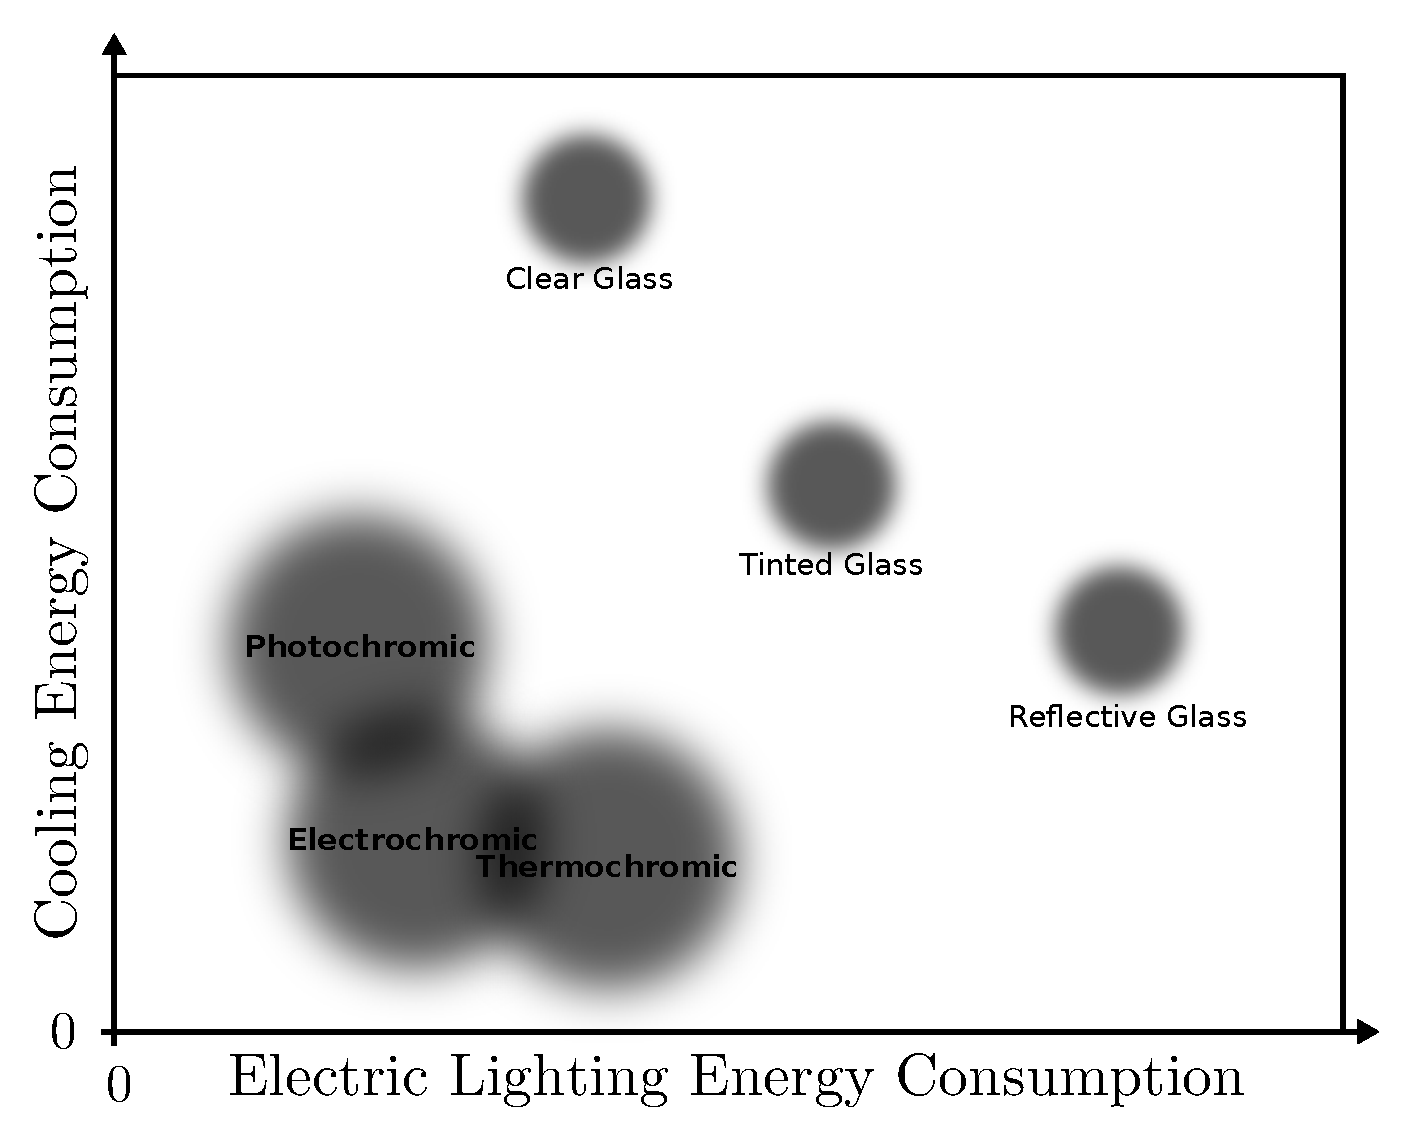
\includegraphics[width=0.5\textwidth]{Figures/chromicGlassComparison.pdf}
   \caption{Comparison of the electric lighting energy and cooling energy consumption between different
   glazing types. Adapted from (\cite{Kamalisarvestani2013},24). \textit{CHECK THIS!!: I understand
      that this graph shows the energy consumption of buildings using using different
      glazing for their windows, i.e. the window glazing impact of the building energy consumption; CHECK END.
      Also, I just drew the graph as good as I could from Kamalisarvestani2013. Is it still okay to use it?
      Should I comment on it not being exact (in case someone try to use data or something, I don't know)?}
   }
\end{figure}
%
\begin{figure}[h!]
  \centering
   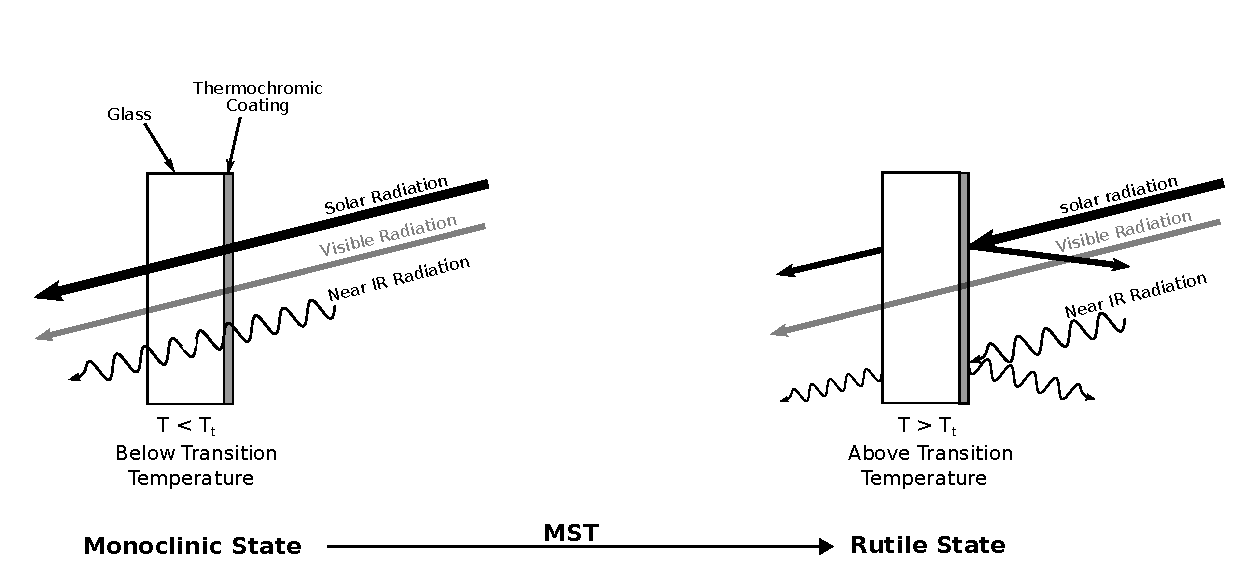
\includegraphics[width=0.9\textwidth]{Figures/TCcoating2.pdf}
   \caption{Schematic representation of thermochromic materials applied as an 
   intelligent window coating \cite{Kiria2010}.
   }
\end{figure}
%
%
\begin{figure}[h!]
  \centering
   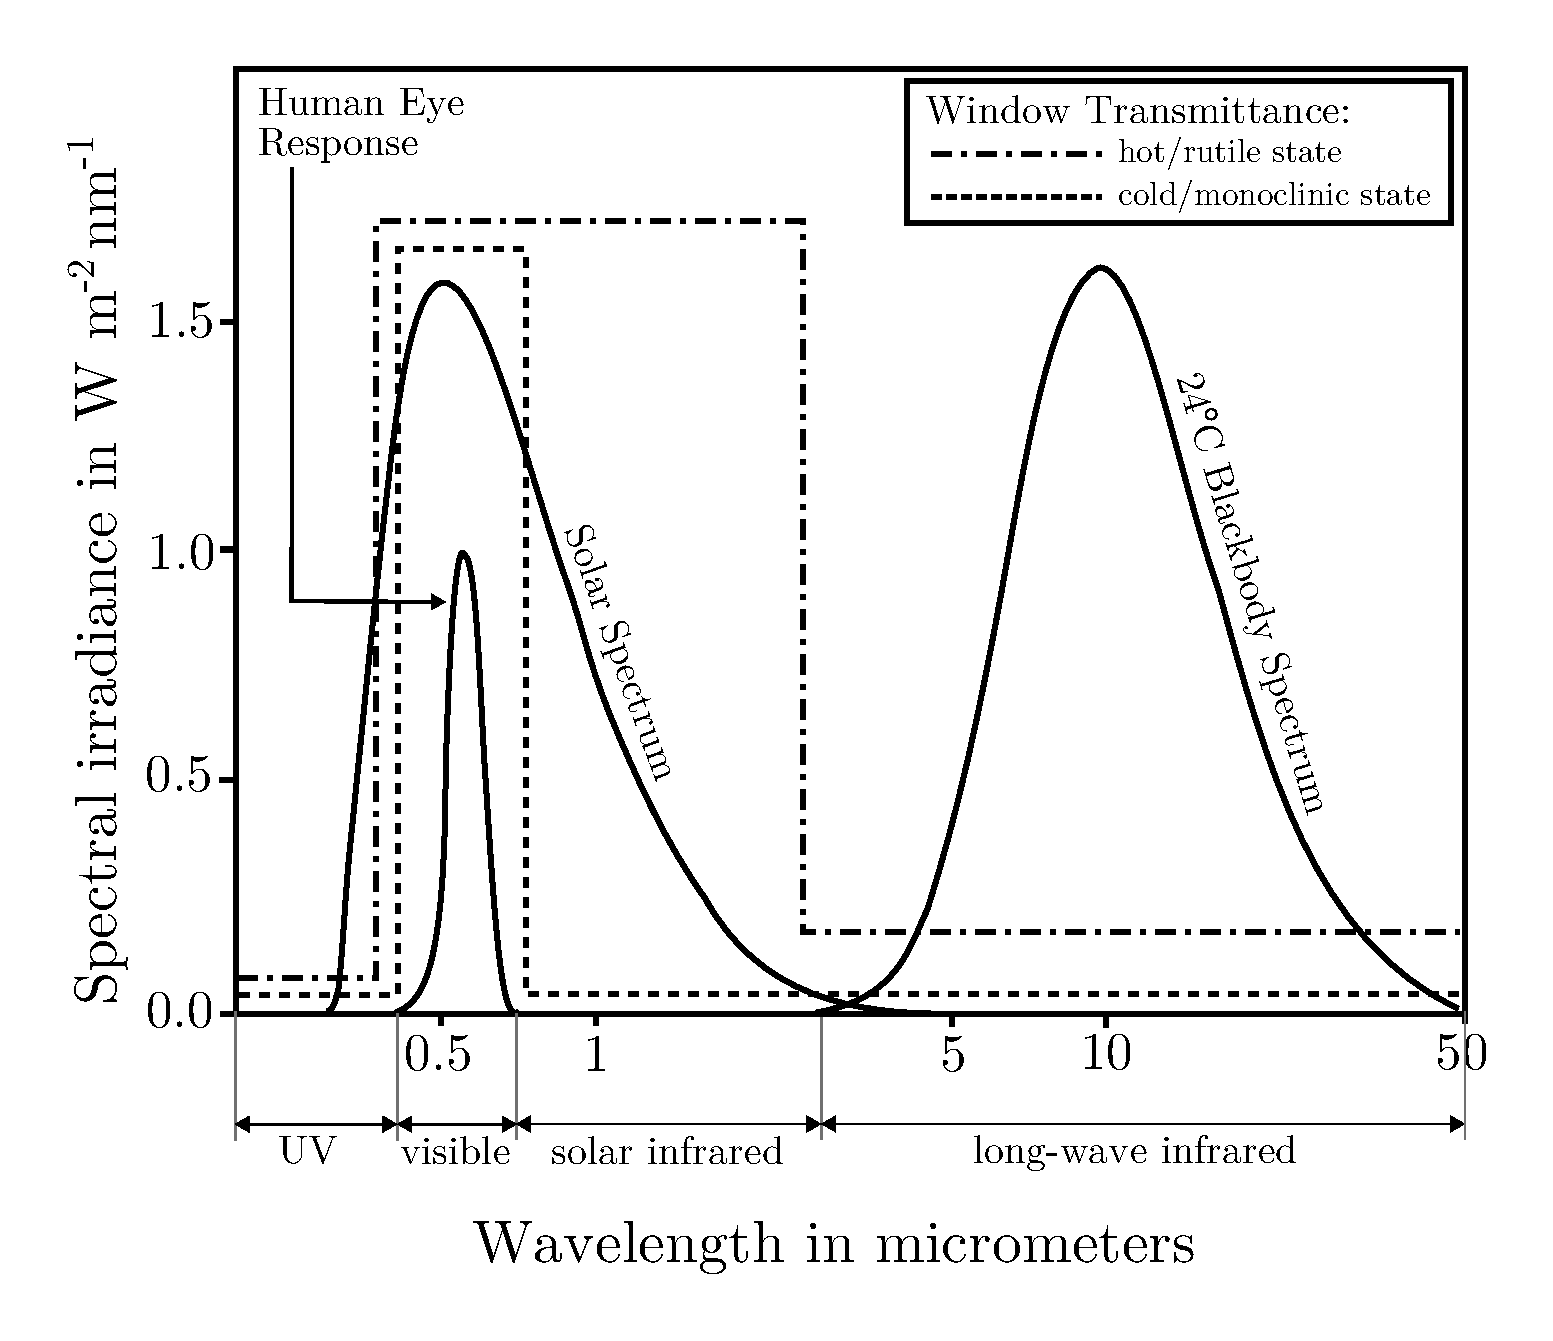
\includegraphics[width=0.5\textwidth]{Figures/TCWtransmittanceMcCluney1996andKamali2013.pdf}
   \caption{The spectral transmittance of a perfect thermochromic window, shown for both 
   cold and hot environments (the monoclinic and rutile state, repsectively). 
   Adopted from \cite{McCluney1996} \cite{Kamalisarvestani2013}
   }
\end{figure}



\textbf{Disposition:}\\
Requirements\\
- Ideal behavior- RADIATION FIGURE and PICTOGRAM\\
- ambient transition temperature\\
- 60\% transmittance in visible range, for lighting\\
-  *Doping\\
-  *Stress/strain\\
-  *thickness\\
\\
- price and mass producable: materials used and current technology\\
\\
Best Candidates:\\
(strengths and weaknesses)\\
-VO2 \\
-etc...\\


\begin{thebibliography}{9}

      \bibitem{McCluney1996}
      McCluney R, Center FSE. 
      Fenestration solar gain analysis. 
      Citeseer 1996.
      
      \bibitem{Kiri2010}
      Kiri P, Hyett G, Binions R.
      Solid state thermochromic materials.
      Advances Material Letters 2010;1(2):20.

\end{thebibliography}


\newpage
\section{Theory}
To understand the theoretical background behind GranFilm and scattering on diffuse surfaces, it is 
convenient to start with the simple case of scattering on a flat interface of two different half-infinite
media, see Figure !!FIGUREREF HERE!!.

The electric permittivity $\varepsilon$ and magnetic permeability $\mu$ of the media are given with subscript $1$ for the above media, and $2$ for the media below. 
Using Maxwell's equations
%
\begin{subequations}
\label{ME}
\begin{align}
   \nabla \cdot \boldsymbol{D} &= \rho \!_f           &\nabla\times\boldsymbol{E} &= - \frac{\partial \boldsymbol{B}}{\partial t} \label{ME1}\\
   \nabla \cdot \boldsymbol{B} &= 0                &\nabla \times \boldsymbol{H}&= \boldsymbol{J}\!_f + \frac{\partial \boldsymbol{D}}{\partial t}, \label{ME2}
\end{align}
\end{subequations}
%
where the electric fields, $\boldsymbol{E}$ and $\boldsymbol{D}$, and magnetic fields $\boldsymbol{B}$ and $\boldsymbol{H}$ are related through
\begin{align}
   &\boldsymbol{D} = \varepsilon \boldsymbol{E},         &\boldsymbol{H} = \frac{1}{\mu} \boldsymbol{B}
\end{align}
(assuming linear media), the fields above $\boldsymbol{E}^+(\boldsymbol{r})$ and below $\boldsymbol{E}^-(\boldsymbol{r})$ the interface can be calculated for a incident place wave 
(same goes for $\boldsymbol{B}$, $\boldsymbol{D}$ and $\boldsymbol{H}$).
So far, the boundary between the two half-infinite media has been considered to be a sharp, flat discontinuity in $\varepsilon(z)$ and $\mu (z)$. 
As soon as the surface roughness, thickness and/or impurities are taken into acount, the complexity of the problem increases.


\textbf{From ''GranFilm-Software-Article''}: \\
Information on the dieletric behavior of surfaes can often be obtained by measuring the Fresnel coefficients,
such as reflection, transmission and absorption. \\
?p.2?: for a layer with thickness negligible compared to wavelength, we introduce surface susceptibilities 
which interconnect the  fresnel coeff. and characterise the optical response of the surface. ?? DID I UNDERSTAND THIS CORRECTLY? ?? \\
Since all the Fresnel coeff. can be expressed in terms of these surface susceptibilities, the main task consist of calculating these coefficients for the appropriate geometry. \\
\textbf{Goal of GranFilm:} to calculate ?surface-susceptibility-/fresnel-coefficients? and the associated measurableFresnel quantities for various surface layer geometries. 
\begin{itemize}
\item GranFilm is free open-source software
\end{itemize}
\subsection{Mie resonances/ plasmon absorption modes}
\textbf{From ''GranFilm-Software-Article''}: \\
when small metallic particles, the resonances can be absorbed by visible light and strongly affect the fresnel 
coefficients depending on the particle morphology.
%
\subsection{Quasistatic Approximation}
%
\subsection{Electromagnetic excess fields }
%
\textbf{From ''GranFilm-Software-Article''}: \\
(Bedeaux and Vlieger) \\
Difference between the bulk extrapolated fields and the real fields. The BC at the dividing surface
(which drive all fresnel coeff.) are given in terms of the integrated excess fields perpendicular to
the surface. \\
Bedeaux and Vlieger $\rightarrow$ formalism of excess quantities (does not require exact knowledge of the near suface EM-field behaviour). \\
Excess fields are defined as the differene between the real fields and the bulk fields extrapolated to the surface. E.g. for the electric field $E(r)$ the excess quantity is defined as
\begin{align}
   E_{ex} (r) = E(r) - E^-(r) \theta(-z) - E^+(r)\theta(z),
\end{align}
where $\theta(z)$ is the Heaviside function and the superscript $\pm$ are used to indicate the region above (+) and below (-) the dividing interface at $z = 0$. 
The excess field is only significant close to the surface, since $E(r, \omega) \rightarrow \rightarrow E^{\pm}(r,\omega)$  for $z \rightarrow \pm \infty$. \\
\textit{QUESTION: \@ Is the $E^{\pm}$ field solved for a infinite homogeneous medium of type (+) and (-) respectively  OR the field in simple two media interface scattering?} \\
\textbf{From Leif Amund Lies Msc Thesis}: \\
Since the excess fields will only be significant close to the surface, they may be thought of as perturbations to the simple case of flat interface. 
\textit{OWN INTERPRETATION: \@ This meas that the bulk fields are the fields created from scattering in the interface between two half-infinite media.} \\
Instead of tediously using the quasi-static-"no source"-BC, the excess fields defined as for the electric field above are inserted into the full Maxwell equations to derive new non-sharp boundary conditions.
The result reads
%
\textbf{From Leif Amund Lies Msc Thesis AND GranFilm-Article}: \\
%
\begin{subequations}
   \label{exFieldBC} % Excess Field Boundary Conditions
\begin{align}
   \big[ \boldsymbol{E}^+_{\parallel} (\boldsymbol{r}) - \boldsymbol{E}^-_{\parallel} (\boldsymbol{r}) \big] \bigg\rvert _{z = 0} 
       &= i \omega \hat{z} \times \! \boldsymbol{M}^s_{\parallel}(\boldsymbol{r}_{\parallel}) \:-\: \nabla\!_{\parallel} P^s_{z}(\boldsymbol{r}_{\parallel}) 
       \label{exFieldBC1} \\ 
   \big[ D^+_{z} (\boldsymbol{r}) - D^-_{z} (\boldsymbol{r}) \big] \bigg\rvert _{z = 0} 
      &= - \nabla\!_{\parallel} \boldsymbol{P}^s_{\parallel}(\boldsymbol{r}_{\parallel}) 
      \label{exFieldBC2} \\ 
   \big[ \boldsymbol{H}^+_{\parallel} (\boldsymbol{r}) - \boldsymbol{H}^-_{\parallel} (\boldsymbol{r}) \big] \bigg\rvert _{z = 0} 
      &= i \omega \hat{z} \times \! \boldsymbol{P}^s_{\parallel}(\boldsymbol{r}_{\parallel}) \:-\: \nabla\!_{\parallel} M^s_{z}(\boldsymbol{r}_{\parallel})  
      \label{exFieldBC3} \\ 
   \big[ B^+_{z} (\boldsymbol{r}) - B^-_{z} (\boldsymbol{r}) \big] \bigg\rvert _{z = 0} 
      &= - \nabla\!_{\parallel} \boldsymbol{M}^s_{\parallel}(\boldsymbol{r}_{\parallel}), 
      \label{exFieldBC4}  
\end{align}
\end{subequations}
%
which is derived in Vlieger and Bedaux's \textit{Optical Properties of Surfaces} (p.21). Here the quantities with superscript $s$ are the so-called excess polarization and magnetization densities
\begin{subequations}
\label{surfQuant} %Surface Quantities
\begin{align}
   \boldsymbol{P}^s(\boldsymbol{r}\!_{\parallel}) &= \big( \boldsymbol{D}^s_{\parallel}(\boldsymbol{r}\!_{\parallel}), \:\: - \varepsilon_0 E^s_{z}(\boldsymbol{r}\!_{\parallel}) \big) \label{surfQuant1}\\
   \boldsymbol{M}^s(\boldsymbol{r}\!_{\parallel}) &= \big( \boldsymbol{B}^s_{\parallel}(\boldsymbol{r}\!_{\parallel}), \:\: - \mu_0 H^s_{z}(\boldsymbol{r}\!_{\parallel}) \big) , \label{surfQuant2}
\end{align}
\end{subequations}
and the quantities on the right hand side are the excess fields integrated along the z-axis,
\begin{subequations}
\label{intExQuant} % integrated excess quantities
\begin{align}
   \boldsymbol{D}^s_{\parallel}(\boldsymbol{r}) &= \!\!\!\!\!\!\!\!\! \int\limits ^{\:\:\:\:\:\:\:\:\:\:+\infty}_{\!\!\!\!\!\!\!\!\!\!\!\!\!\!\!-\infty} \!\!\!\!\!\!\!\!\! d\!z\: \boldsymbol{D}\!_{ex,\parallel}(\boldsymbol{r}),
   &E^s_{z}(\boldsymbol{r}) = \!\!\!\!\!\!\!\!\! \int\limits ^{\:\:\:\:\:\:\:\:\:\:+\infty}_{\!\!\!\!\!\!\!\!\!\!\!\!\!\!\!-\infty} \!\!\!\!\!\!\!\!\! d\!z\: E\!_{ex,z}(\boldsymbol{r}) \label{intExQuant1}\\
   \boldsymbol{B}^s_{\parallel}(\boldsymbol{r}) &= \!\!\!\!\!\!\!\!\! \int\limits ^{\:\:\:\:\:\:\:\:\:\:+\infty}_{\!\!\!\!\!\!\!\!\!\!\!\!\!\!\!-\infty} \!\!\!\!\!\!\!\!\! d\!z\: \boldsymbol{B}\!_{ex,\parallel}(\boldsymbol{r}),
   &H^s_{z}(\boldsymbol{r}) = \!\!\!\!\!\!\!\!\! \int\limits ^{\:\:\:\:\:\:\:\:\:\:+\infty}_{\!\!\!\!\!\!\!\!\!\!\!\!\!\!\!-\infty} \!\!\!\!\!\!\!\!\! d\!z\: H\!_{ex,z}(\boldsymbol{r}). \label{intExQuant2}
\end{align}
\end{subequations}
\textit{OWN INTERPRETATION: These integrated excess quantities are equivalent of representing the the excess fields in a single Dirac term $\delta (z)$ located at the surface ($z = 0$), e.g. such that the electric field can be 
written as}
%
\begin{align}
   E(r) =  E^-(r) \theta(-z) + E^s(r)\delta (z) +  E^+(r)\theta(z).
\end{align}
%
\textit{OWN INTERPRETATION: Demanding that this fullfuls Maxwell's Equations, one obtains the Equations in \eqref{exFieldBC} }.
\textit{OWN INTERPRETATION: The simplest way to link the Surface polarization and magnetization density to the extrapolated bulk fields(?Sigma indexed fields?)involves a
symmetric constitutive tensor $\xi^s_e(\omega)$ (ref B,V-OPoS).}
\begin{align}
   \boldsymbol{P}^s(\boldsymbol{r}\!_{\parallel}) = \xi ^s_e \: \big[ \boldsymbol{E}_{\parallel, \Sigma}(\boldsymbol{r}\!_{\parallel}), \:\: - D\!_{z, \Sigma}(\boldsymbol{r}\!_{\parallel}) \big]
\end{align}
\textit{OWN INTERPRETATION: The above relation is restricted to non-magnetic materials, i.e. that $\boldsymbol{M}^s(\boldsymbol{r}\!_{\parallel}) = 0$.   The $\Sigma$ index denotes the arithmetic mean of the upper and lower
bulk fields, e.g. $ \boldsymbol{E}_{\parallel, \Sigma} = \big\{ \boldsymbol{E}^+_{\parallel} \!( \boldsymbol{r}\!_{\parallel} ) +  \boldsymbol{E}^-_{\parallel} \! (\boldsymbol{r}\!_{\parallel}) \big\} \big/2 $.
If the interface are z = 0 is isotropic and symmetric, the interfacial tensor $\xi ^s_e$ is diagonal}:
\begin{align}
\xi ^s_e = 
\begin{bmatrix}
   \gamma   &   0       &  0      \\
   0        &   \gamma  &  0      \\
   0        &   0       &  \beta 
\end{bmatrix}
.
\end{align}
Here the coefficients $\gamma$ and $\beta$ are called the (first-order) surface susceptibilities (or here, constitutive coefficients). The constitutive coefficients of second order, $\delta$ and $\tau$ describe
a non-local dependence (??SPATIAL VARIATIONS IN THE EXCESS QUANTITIES??) \\
\textbf{Fresnel Coefficients} \\
...need to write some more here...
\begin{subequations}
   \label{fresCoeffS}
\begin{align}
   r_s(\omega) &= \frac{n\!_{_-} \cos \theta_i - n\!_{_+} \cos \theta_t + i(\omega/c) \gamma}{n\!_{_-} \cos \theta_i + n\!_{_+} \cos \theta_t - i(\omega/c) \gamma} \label{fresCoeffS1} \\
   t_s(\omega) &= \frac{2 n\!_{_-} \cos \theta_i}{n\!_{_-} \cos \theta_i + n\!_{_+} \cos \theta_t - i(\omega/c) \gamma} \label{fresCoeffS2}
\end{align}
\end{subequations}
%
\begin{subequations}
\label{fresCoeffP}
\begin{align}
   r_p(\omega) &= \frac{\kappa\!_{_-}(\omega) -i(\omega / c) \gamma \cos \theta_i \cos \theta_t + i(\omega/c)n\!_{_-} n\!_{_+} \varepsilon\!_{_-}\beta\sin^2 \theta_i }
   {\kappa\!_{_+}(\omega) -i(\omega / c) \gamma \cos \theta_i \cos \theta_t - i(\omega/c) n\!_{_-} n\!_{_+} \varepsilon\!_{_-} \beta \sin^2 \theta_i }, \label{fresCoeffS1}\\
   t_p(\omega) &= \frac{2n\!_{_-} \cos \theta_i \big[ 1 + (\omega/2c)^2 \varepsilon\!_{_-} \gamma \beta \sin ^2 \theta_i \big]}
   {\kappa\!_{_+}(\omega) -i(\omega / c) \gamma \cos \theta_i \cos \theta_t - i(\omega/c) n\!_{_-} n\!_{_+} \varepsilon\!_{_-} \beta \sin^2 \theta_i }, \label{fresCoeffS2}\\
   \kappa\!_{\pm} &= \big[ n\!_{_+} \cos \theta _i \pm n\!_{_-} \cos \theta_t  \big]\Bigg[ 1 - \frac{\omega^2}{4c^2} \varepsilon\!_{_-} \gamma \beta \sin ^2 \theta_i \Bigg]. \label{fresCoeffS3}
\end{align}
\end{subequations}
%
%\begin{subequations}
%\begin{align}
   %r_p(\omega) &= \frac{\kappa _-(\omega) -i(\omega / c) \gamma \cos \theta_i \cos \theta_t + i(\omega/c)n_-n_+\varepsilon_-\beta\sin^2 \theta_i }
               %{\kappa _+(\omega) -i(\omega / c) \gamma \cos \theta_i \cos \theta_t - i(\omega/c)n_-n_+\varepsilon_-\beta\sin^2 \theta_i } \\
   %t_p(\omega) &= \frac{2n_- \cos \theta_i \big[ 1 + (\omega/2c)^2 \varepsilon_- \gamma \beta \sin ^2 \theta_i \big]}
               %{\kappa _+(\omega) -i(\omega / c) \gamma \cos \theta_i \cos \theta_t - i(\omega/c)n_-n_+\varepsilon_-\beta\sin^2 \theta_i } \\
   %\kappa_{\pm} &= \big[ n_+ \cos \theta _i \pm n_- \cos \theta_t  \big]\Bigg[ 1 - \frac{\omega^2}{4c^2} \varepsilon_- \gamma \beta \sin ^2 \theta_i \Bigg]
%\end{align}
%\end{subequations}
From Eq. \eqref{fresCoeff1}-Eq.\eqref{fresCoeff3} we can observe that $p$-polarized excite the surface in both parallel and perpendicular direction, relative to the surface. 






\subsection{.}


\textbf{D'Alembert Operator $\square$}
\begin{align*}
  \square  &= \partial ^{\mu} \partial _{\mu}
   \\
           &= \frac{1}{c^2} \frac{\partial ^2}{\partial t^2} 
               - \frac{\partial ^2}{\partial x^2} 
               - \frac{\partial ^2}{\partial y^2} 
               - \frac{\partial ^2}{\partial z^2} 
   \\
           &= \frac{1}{c^2} \frac{\partial ^2}{\partial t^2} - \nabla ^2
\end{align*}

\textbf{Lorentz Gauge:} \\
For Lorentz invariance, convenient to choose the Lorenz gauge:
\begin{align*}
   \square \vec{A} = \Bigg[ \frac{1}{c^2} \frac{\partial ^2}{\partial t^2} - \nabla ^2 \Bigg] \vec{A} = \mu_0 \vec{J}
\end{align*}
\begin{align*}
   \square \phi = \Bigg[ \frac{1}{c^2} \frac{\partial ^2}{\partial t^2} - \nabla ^2 \Bigg] \phi = \frac{\rho}{\epsilon _0}
\end{align*}



\newpage
\section{Method}

\section{Results}
The following simulations are done with an incident plane wave of direction 
$(\theta_i,\phi_i) = (45^{\circ},0^{\circ})$, on VO$_2$ particles supported by a SiO$_2$ substrate
with truncation ratio $t_r = 0$. The surrounding medium is air with $\varepsilon(\omega,T) = 1$.
The particles are arranged in a square lattice with lattice constant $L = 45$nm and the
particle-particle interaction is given by a dipole contribution. The multipole truncation
is set to $M = 16$.
\section{Simulation 1; $R = 10$nm, p-polarized incident light}
%
\begin{figure}
    \centering
    \begin{subfigure}[b]{0.49\textwidth}
        \centering
        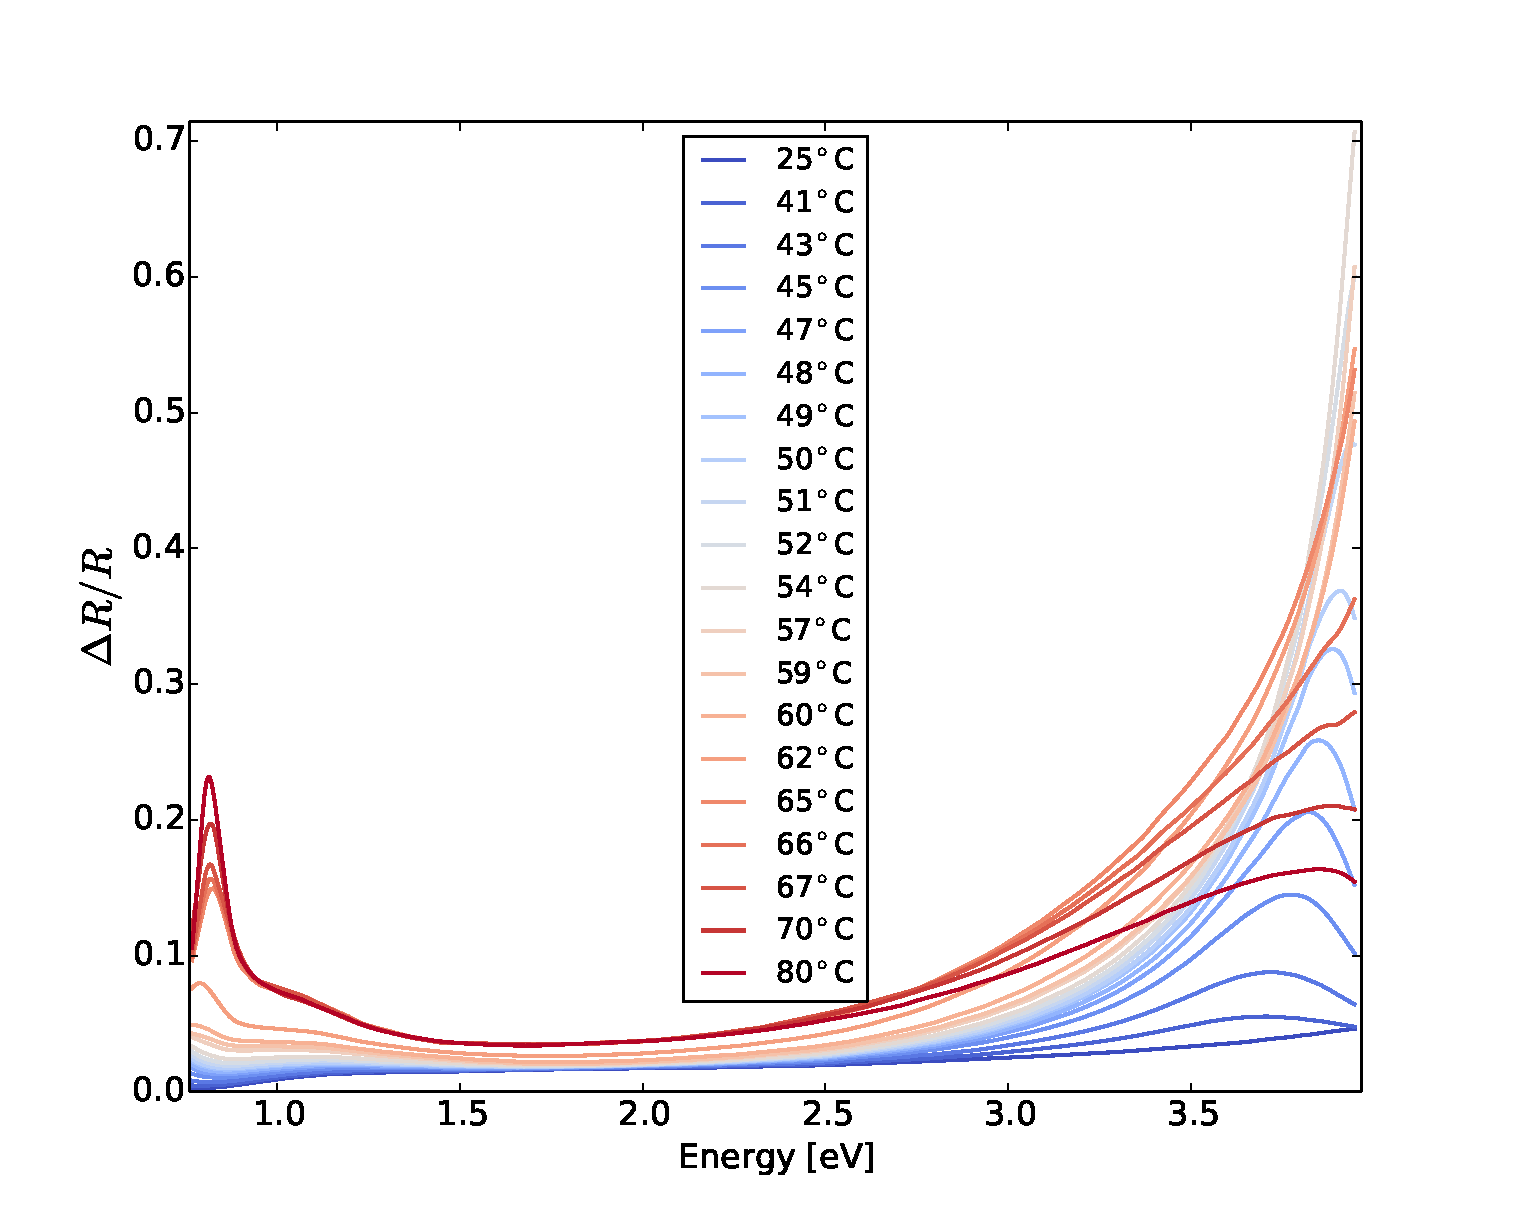
\includegraphics[width=\textwidth]{Results/Sim1/dR.pdf}
        \caption{}
        \label{fig:}
    \end{subfigure}
    %\hfill
    \begin{subfigure}[b]{0.49\textwidth}
        \centering
        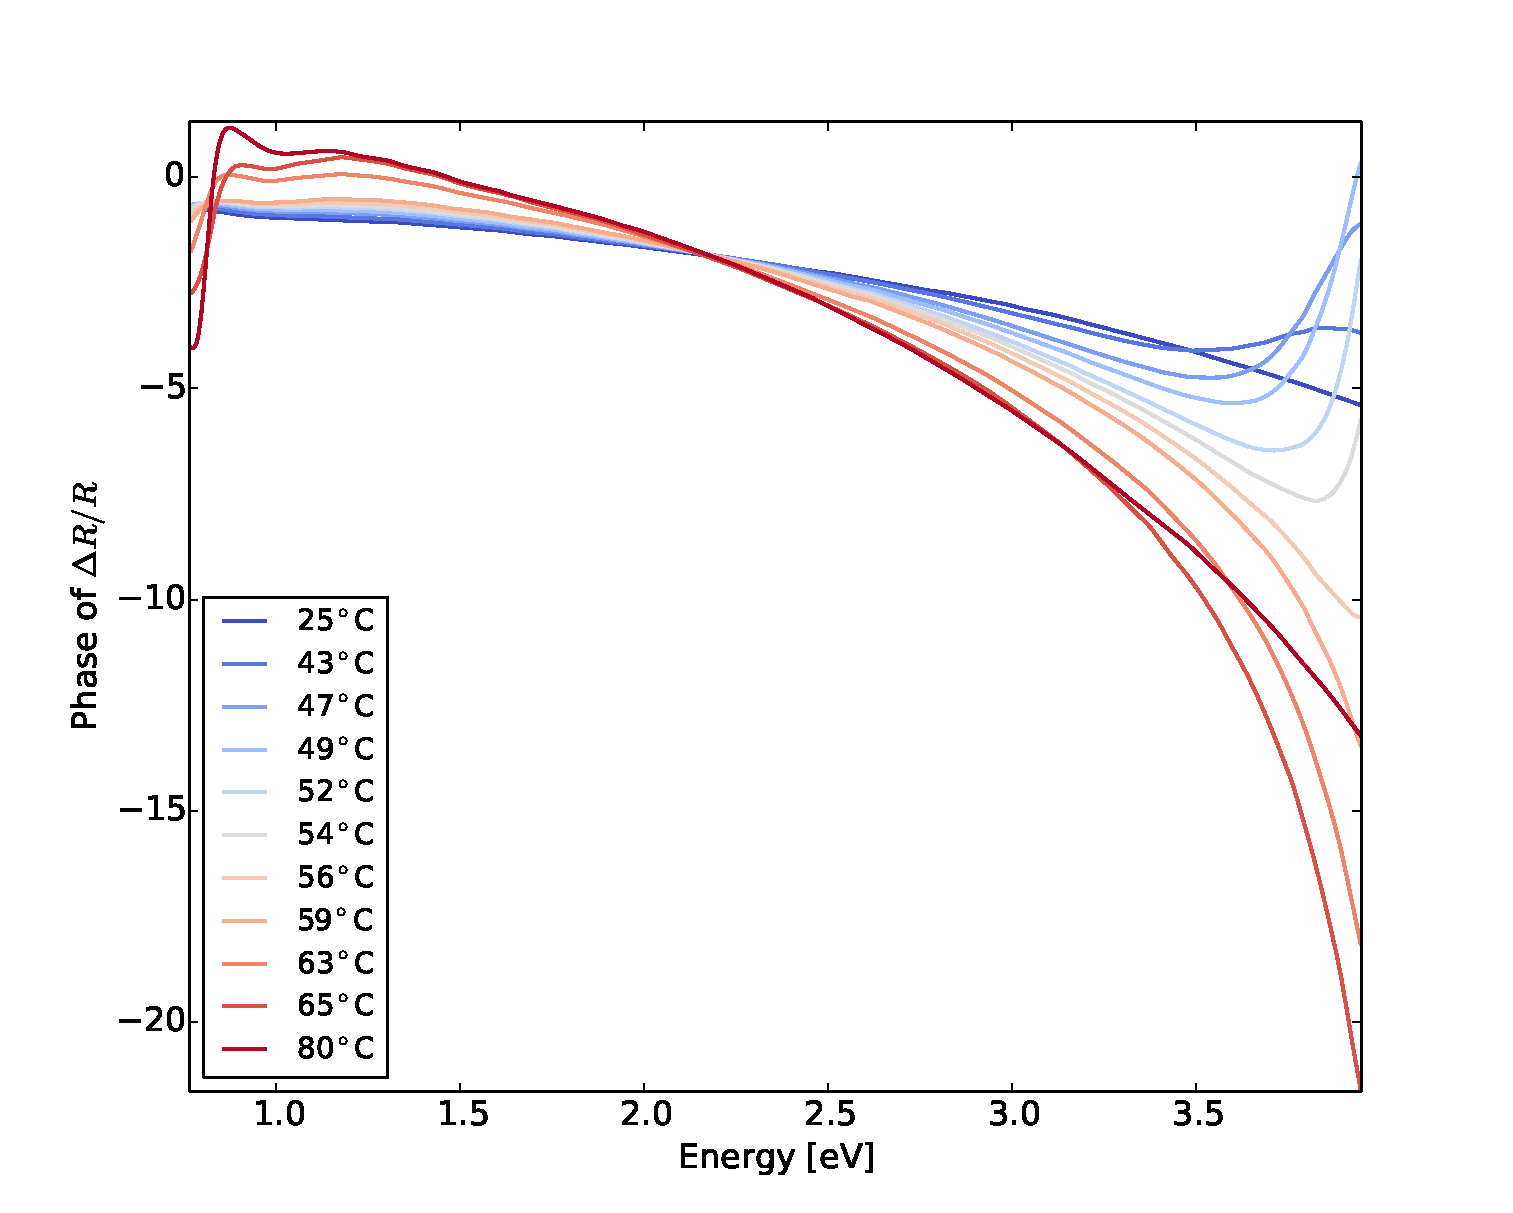
\includegraphics[width=\textwidth]{Results/Sim1/dRphase.pdf}
        \caption{}
        \label{fig:}
    \end{subfigure}
    \caption{Relative reflectance $\Delta R/R$}
    \label{fig:1}
\end{figure}
%
%
\begin{figure}
    \centering
    \begin{subfigure}[b]{0.49\textwidth}
        \centering
        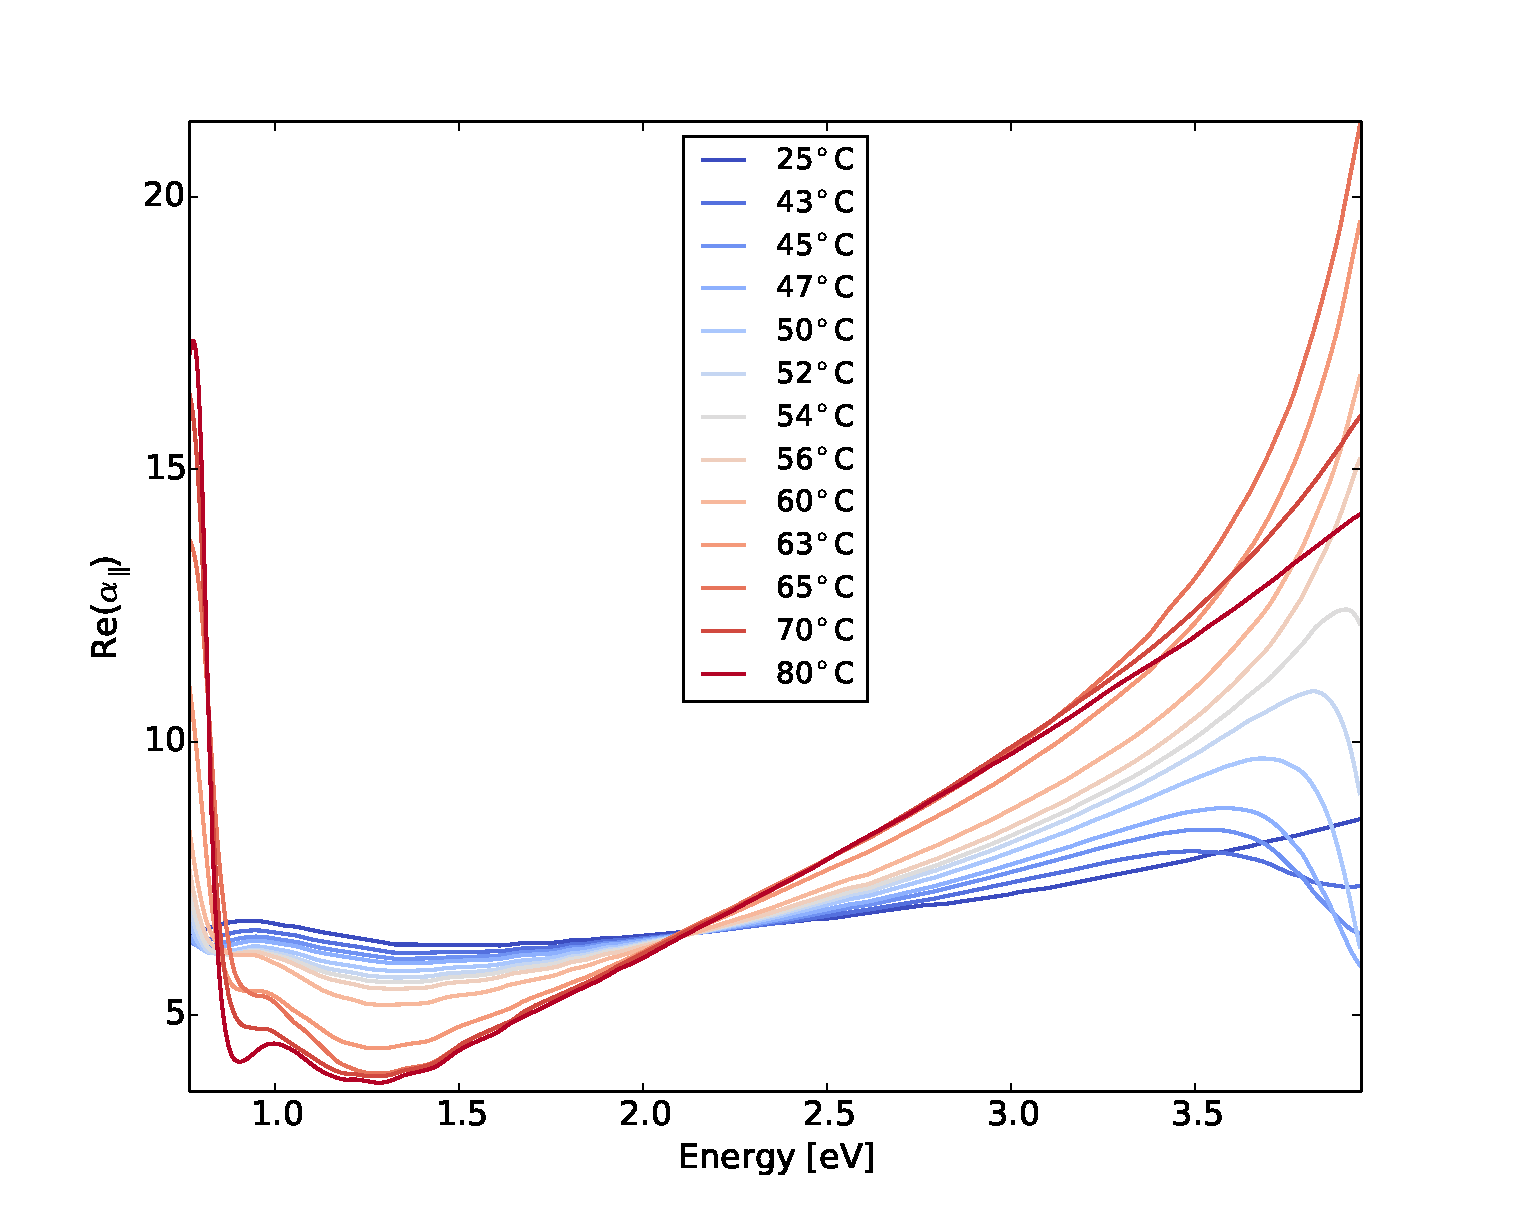
\includegraphics[width=\textwidth]{Results/Sim1/re_alpha_parallel.pdf}
        \caption{}
        \label{fig:2}
    \end{subfigure}
    %\hfill
    \begin{subfigure}[b]{0.49\textwidth}
        \centering
        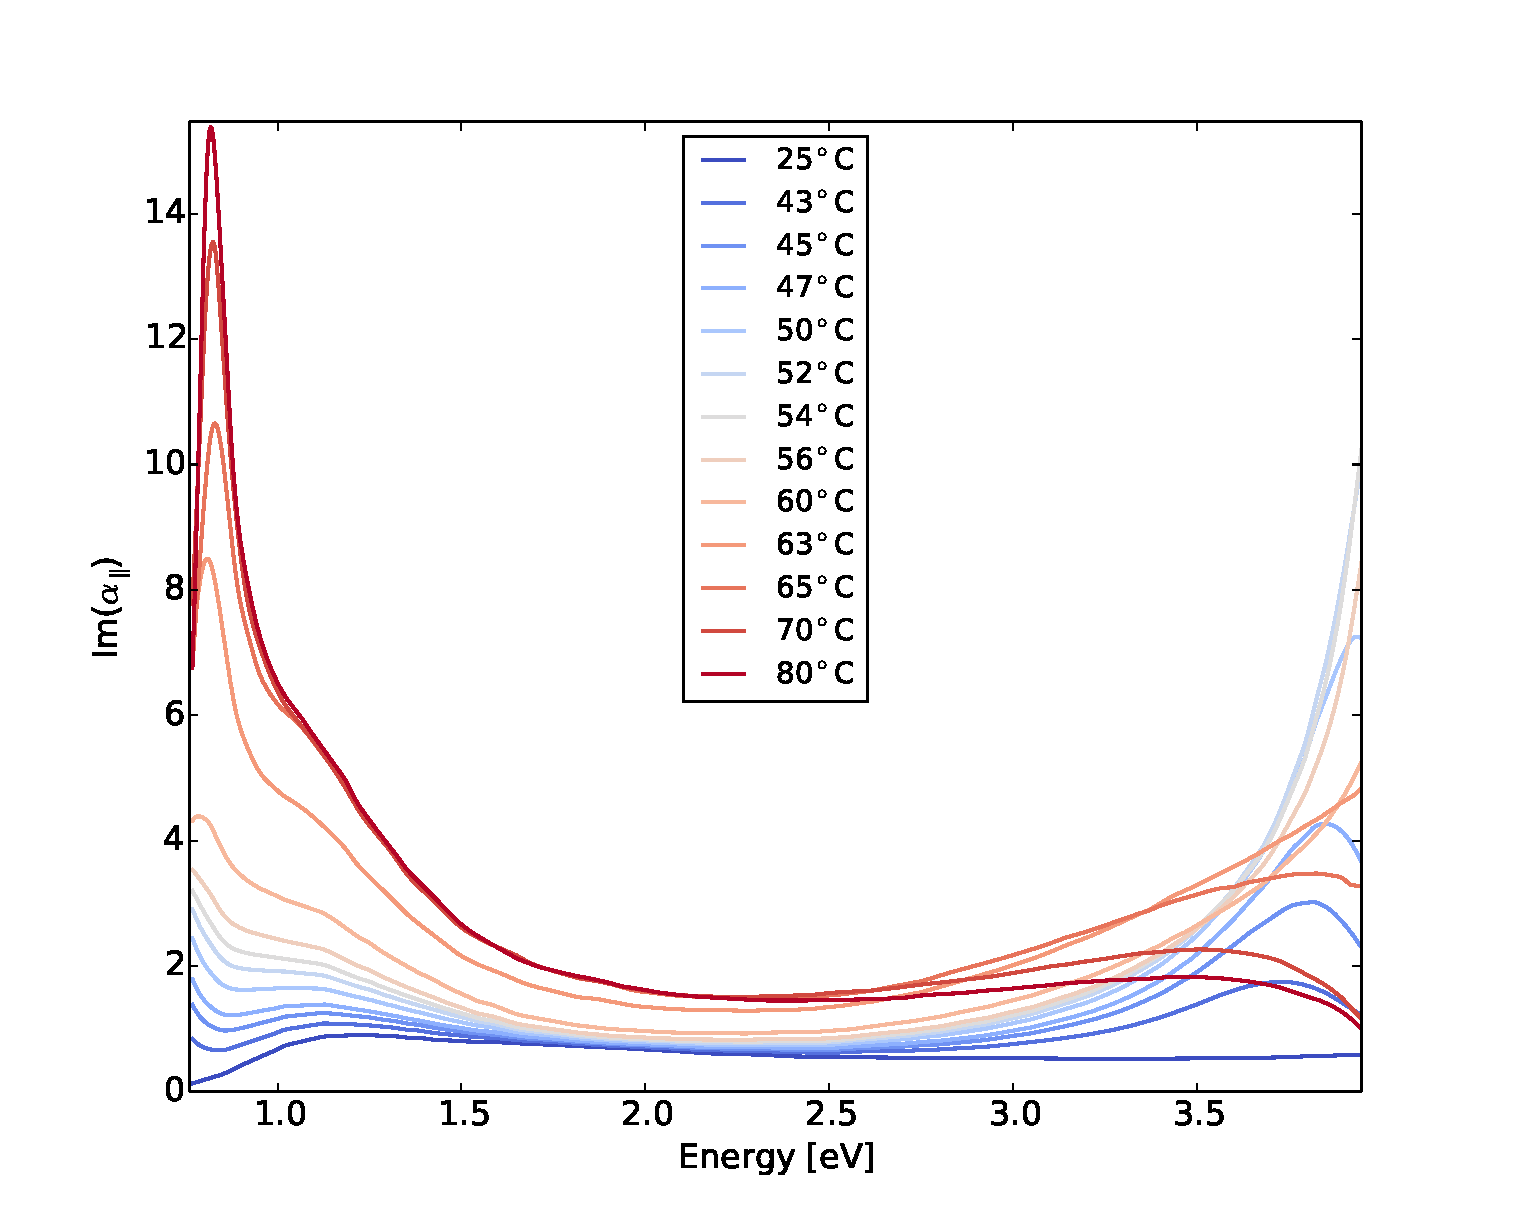
\includegraphics[width=\textwidth]{Results/Sim1/im_alpha_parallel.pdf}
        \caption{}
        \label{fig:2}
    \end{subfigure}
    %\hfill
    \begin{subfigure}[b]{0.49\textwidth}
        \centering
        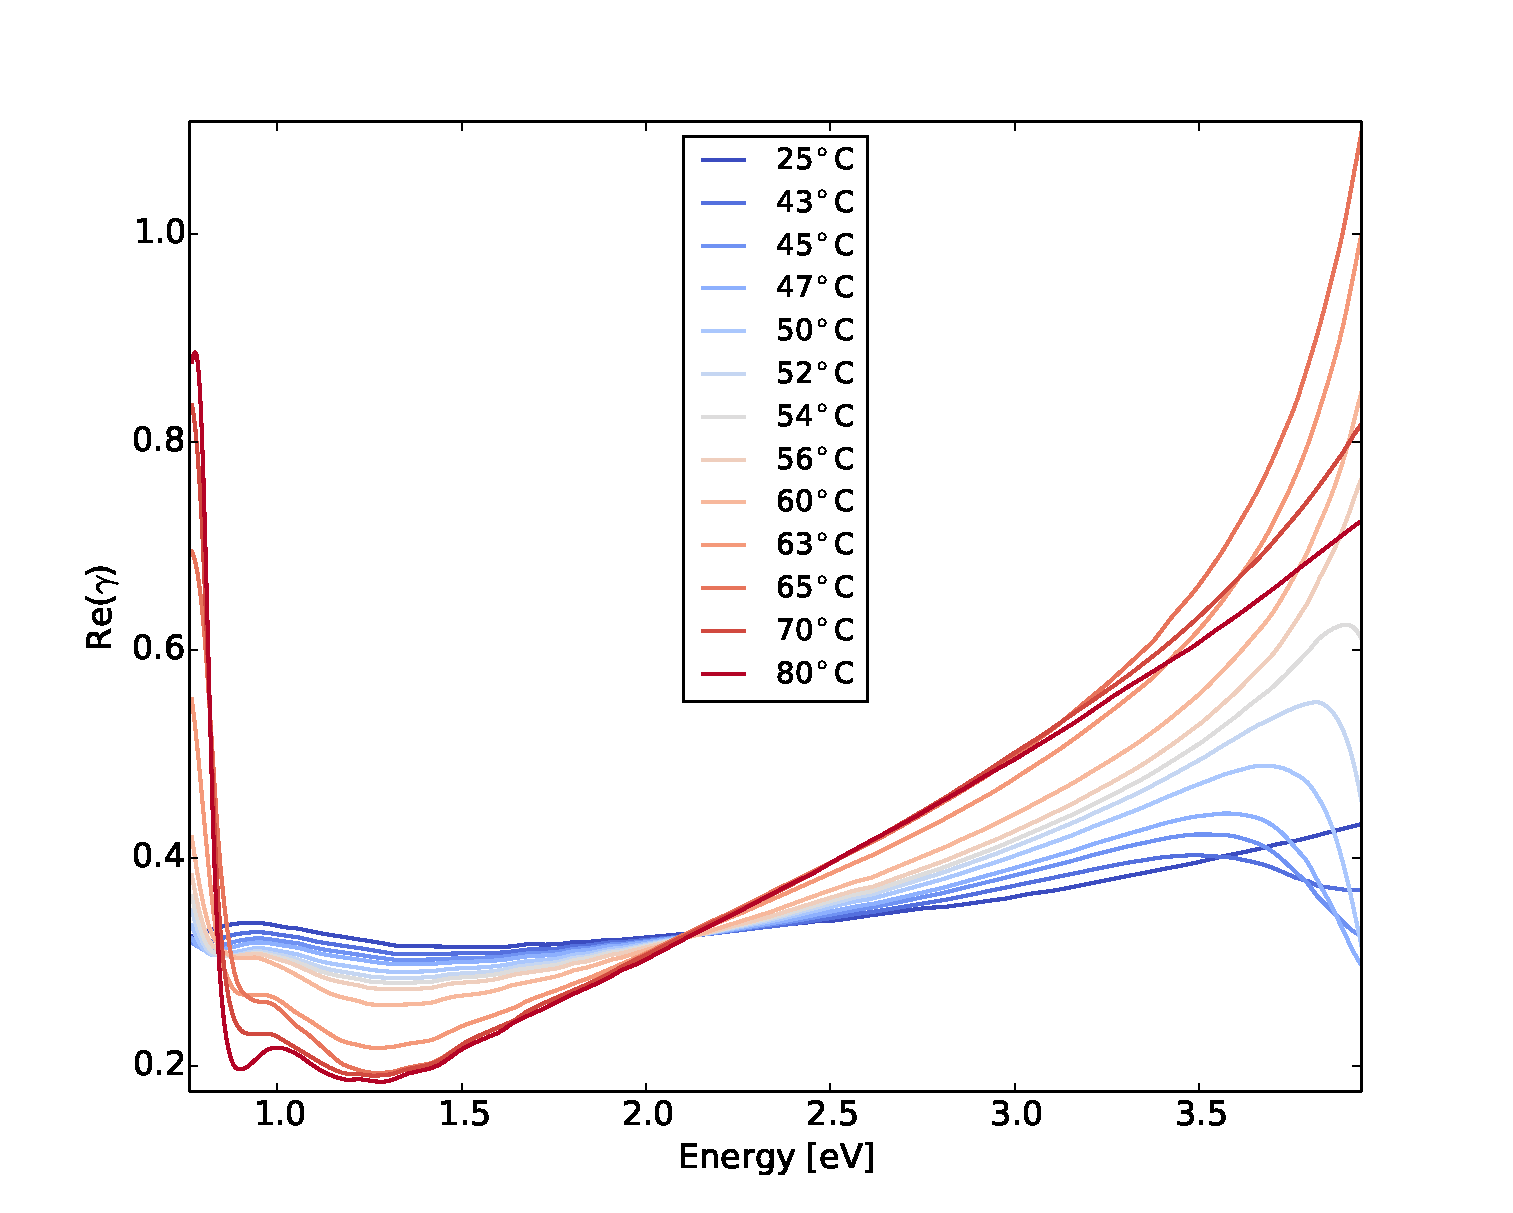
\includegraphics[width=\textwidth]{Results/Sim1/re_gamma.pdf}
        \caption{}
        \label{fig:2}
    \end{subfigure}
    %\hfill
    \begin{subfigure}[b]{0.49\textwidth}
        \centering
        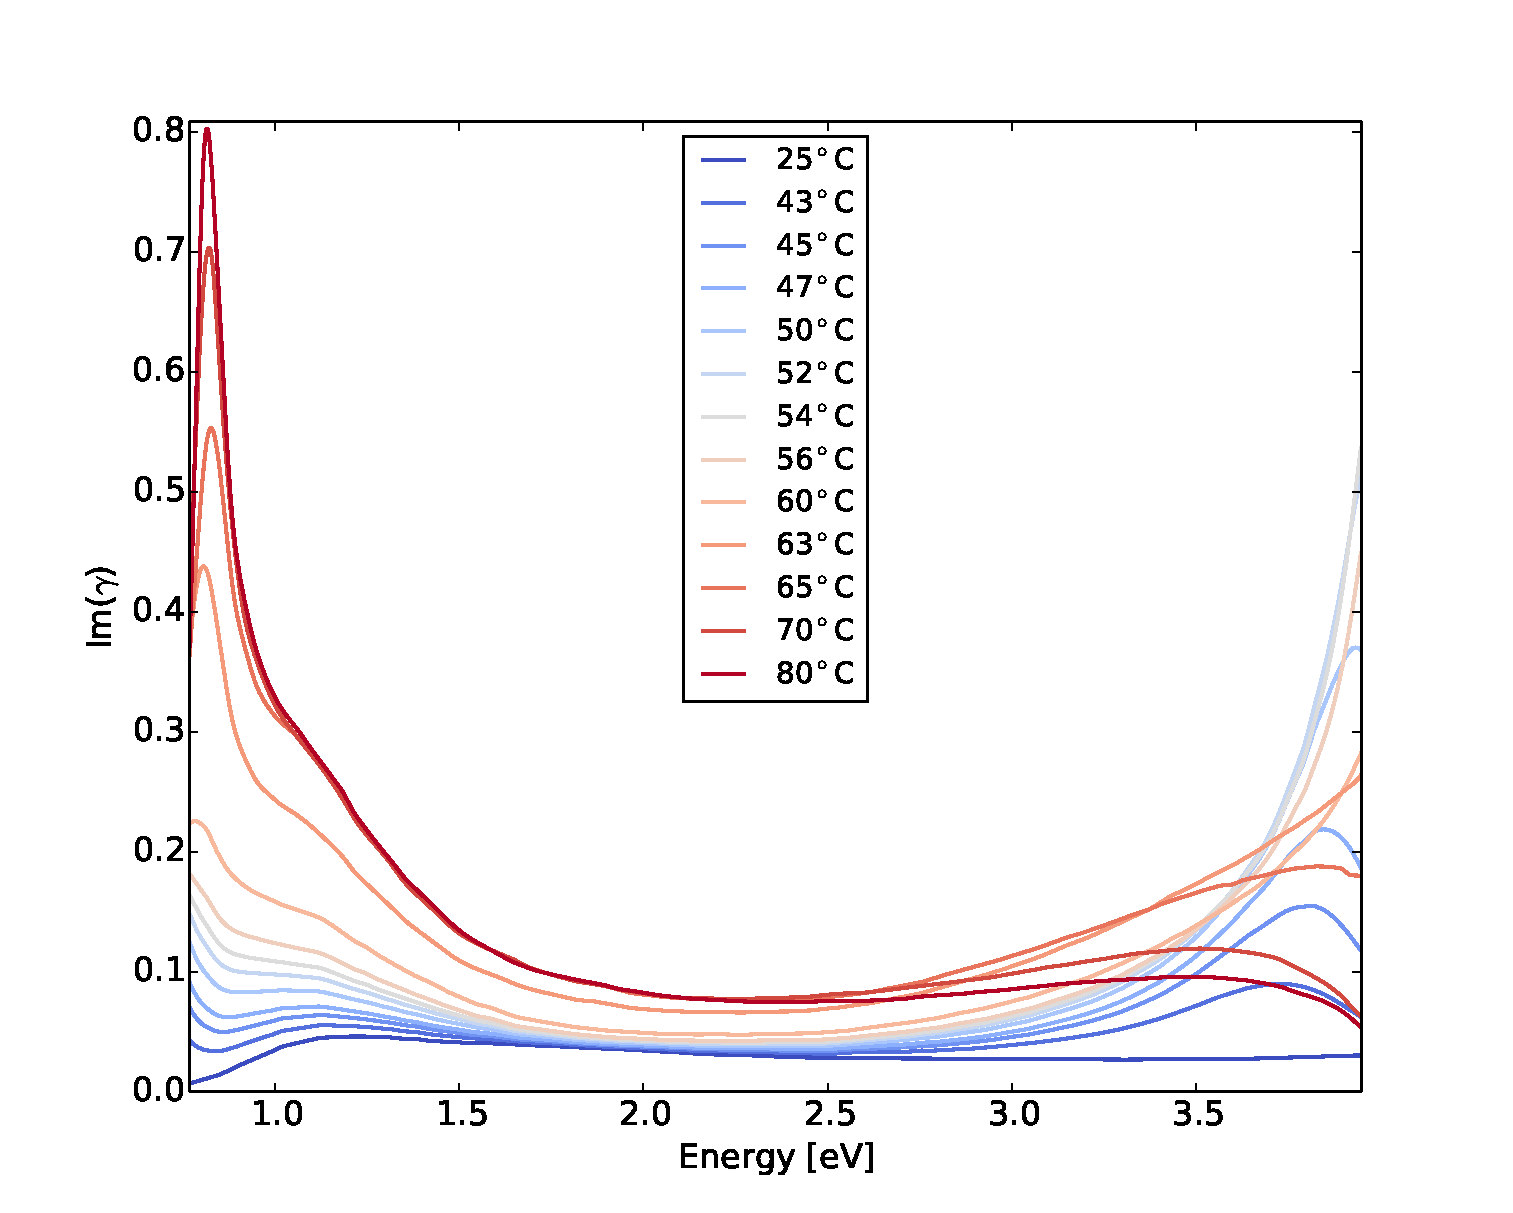
\includegraphics[width=\textwidth]{Results/Sim1/im_gamma.pdf}
        \caption{}
        \label{fig:2}
    \end{subfigure}
    \caption{Relative reflectance $\Delta R/R$}
    \label{fig:}
\end{figure}
%
%
\begin{figure}
    \centering
    \begin{subfigure}[b]{0.49\textwidth}
        \centering
        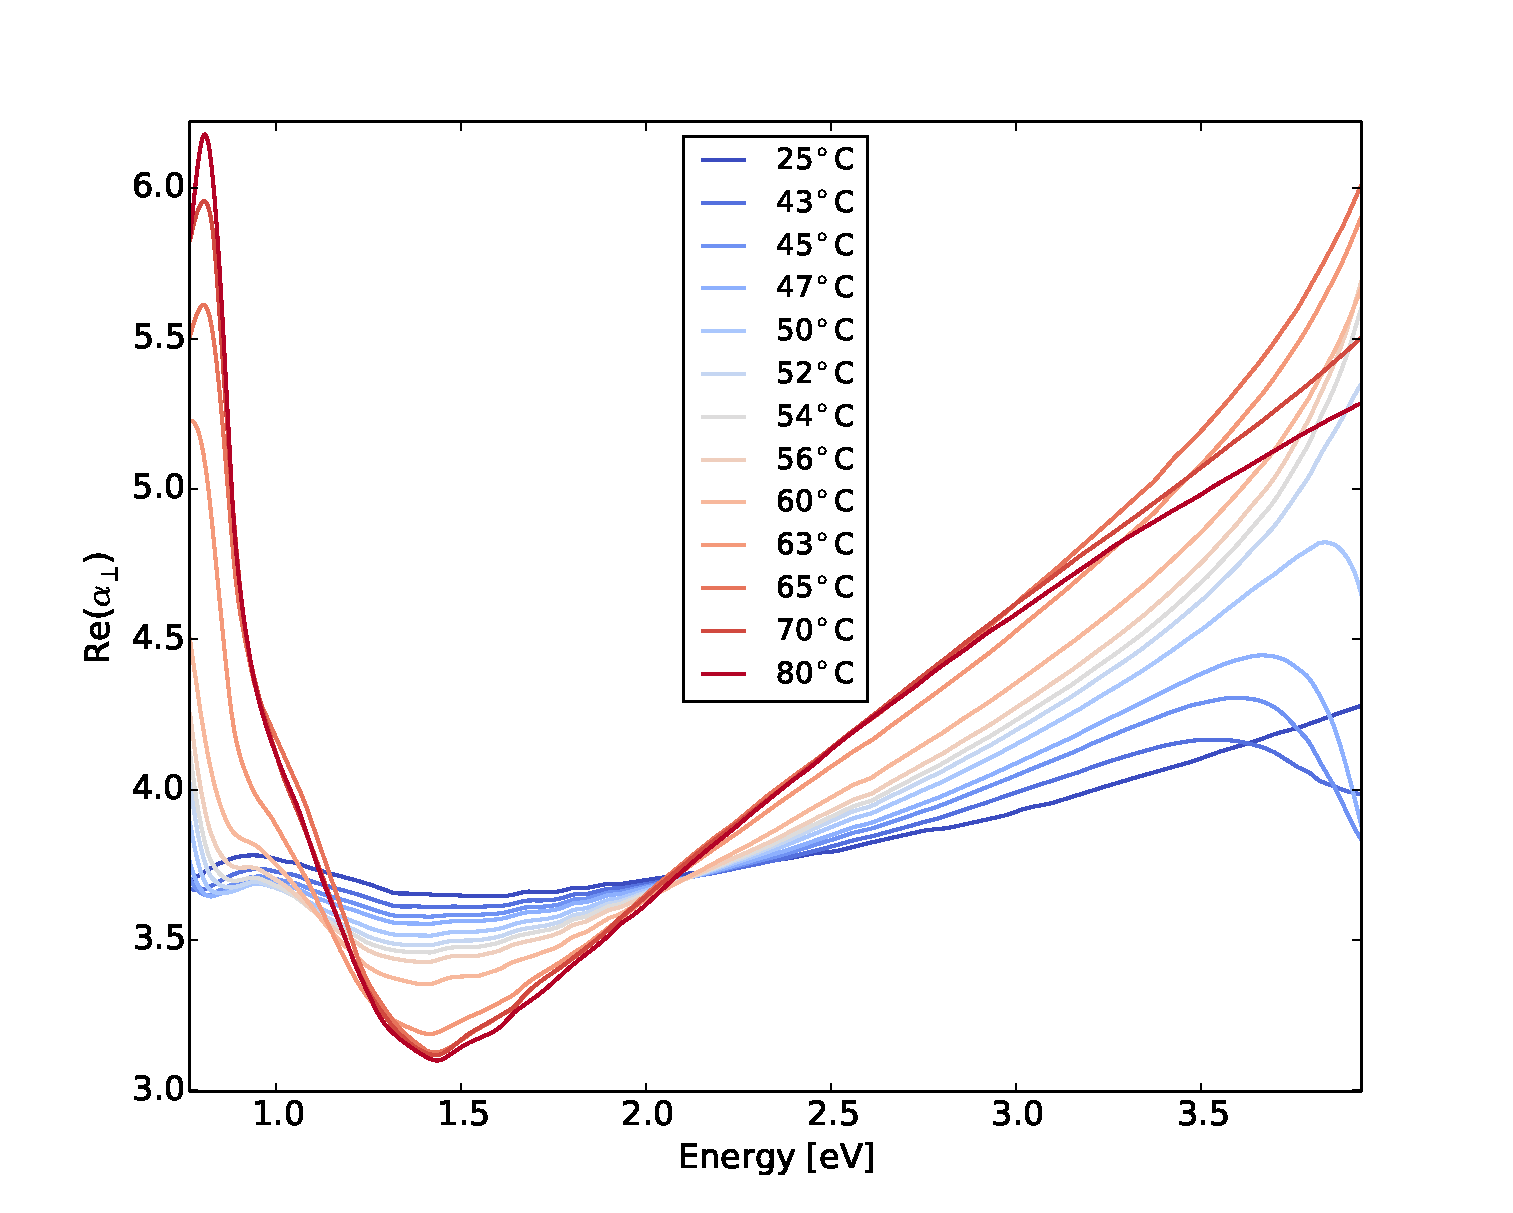
\includegraphics[width=\textwidth]{Results/Sim1/re_alpha_perp.pdf}
        \caption{}
        \label{fig:}
    \end{subfigure}
    %\hfill
    \begin{subfigure}[b]{0.49\textwidth}
        \centering
        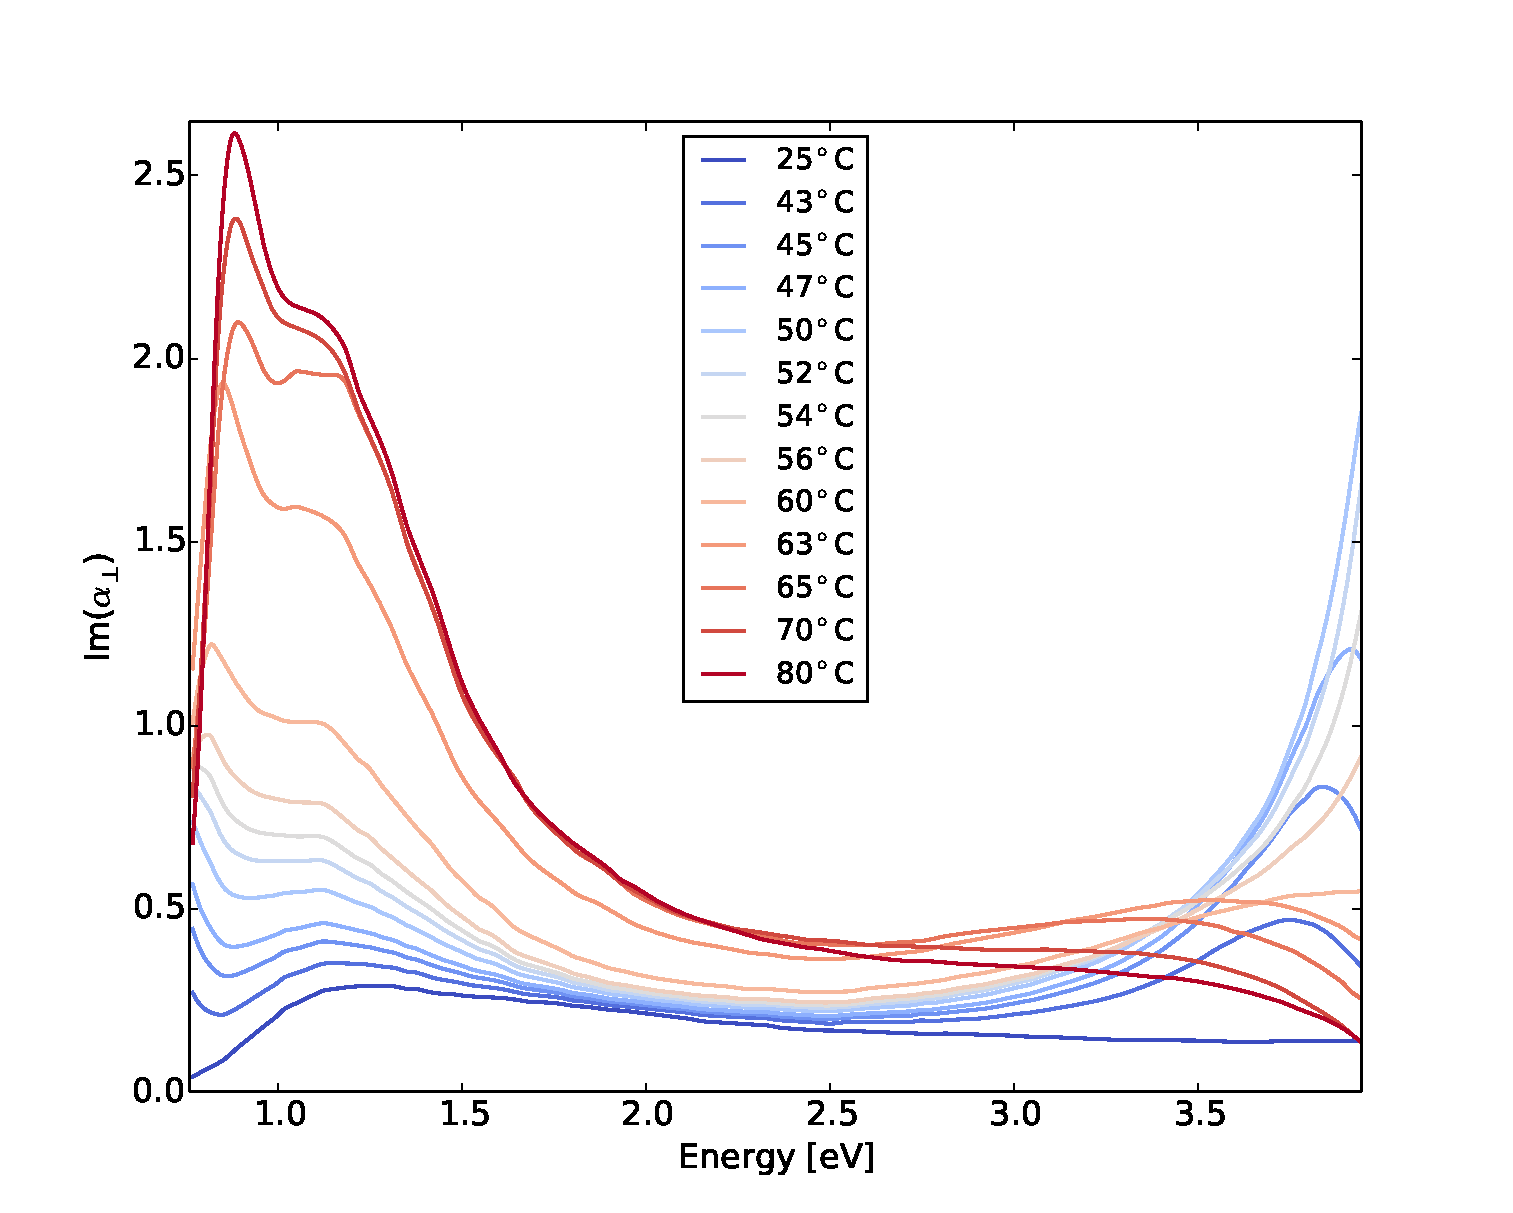
\includegraphics[width=\textwidth]{Results/Sim1/im_alpha_perp.pdf}
        \caption{}
        \label{fig:}
    \end{subfigure}
    %\hfill
    \begin{subfigure}[b]{0.49\textwidth}
        \centering
        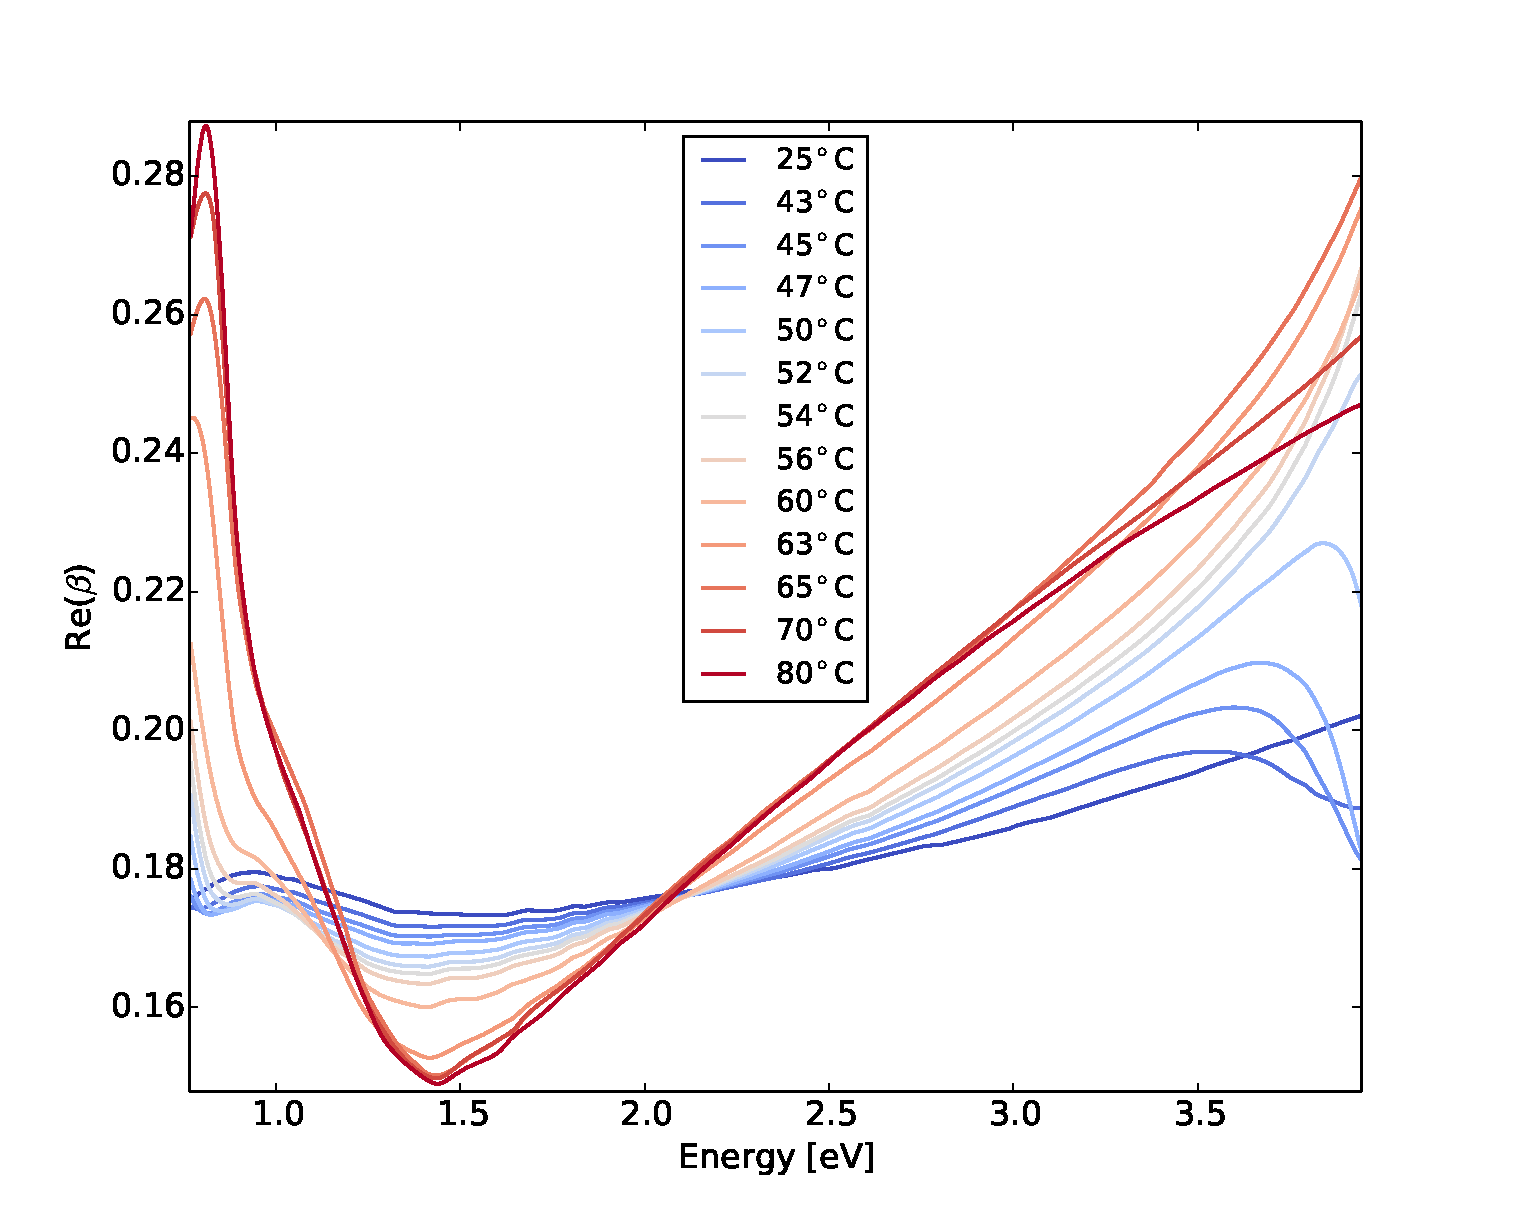
\includegraphics[width=\textwidth]{Results/Sim1/re_beta.pdf}
        \caption{}
        \label{fig:2}
    \end{subfigure}
    %\hfill
    \begin{subfigure}[b]{0.49\textwidth}
        \centering
        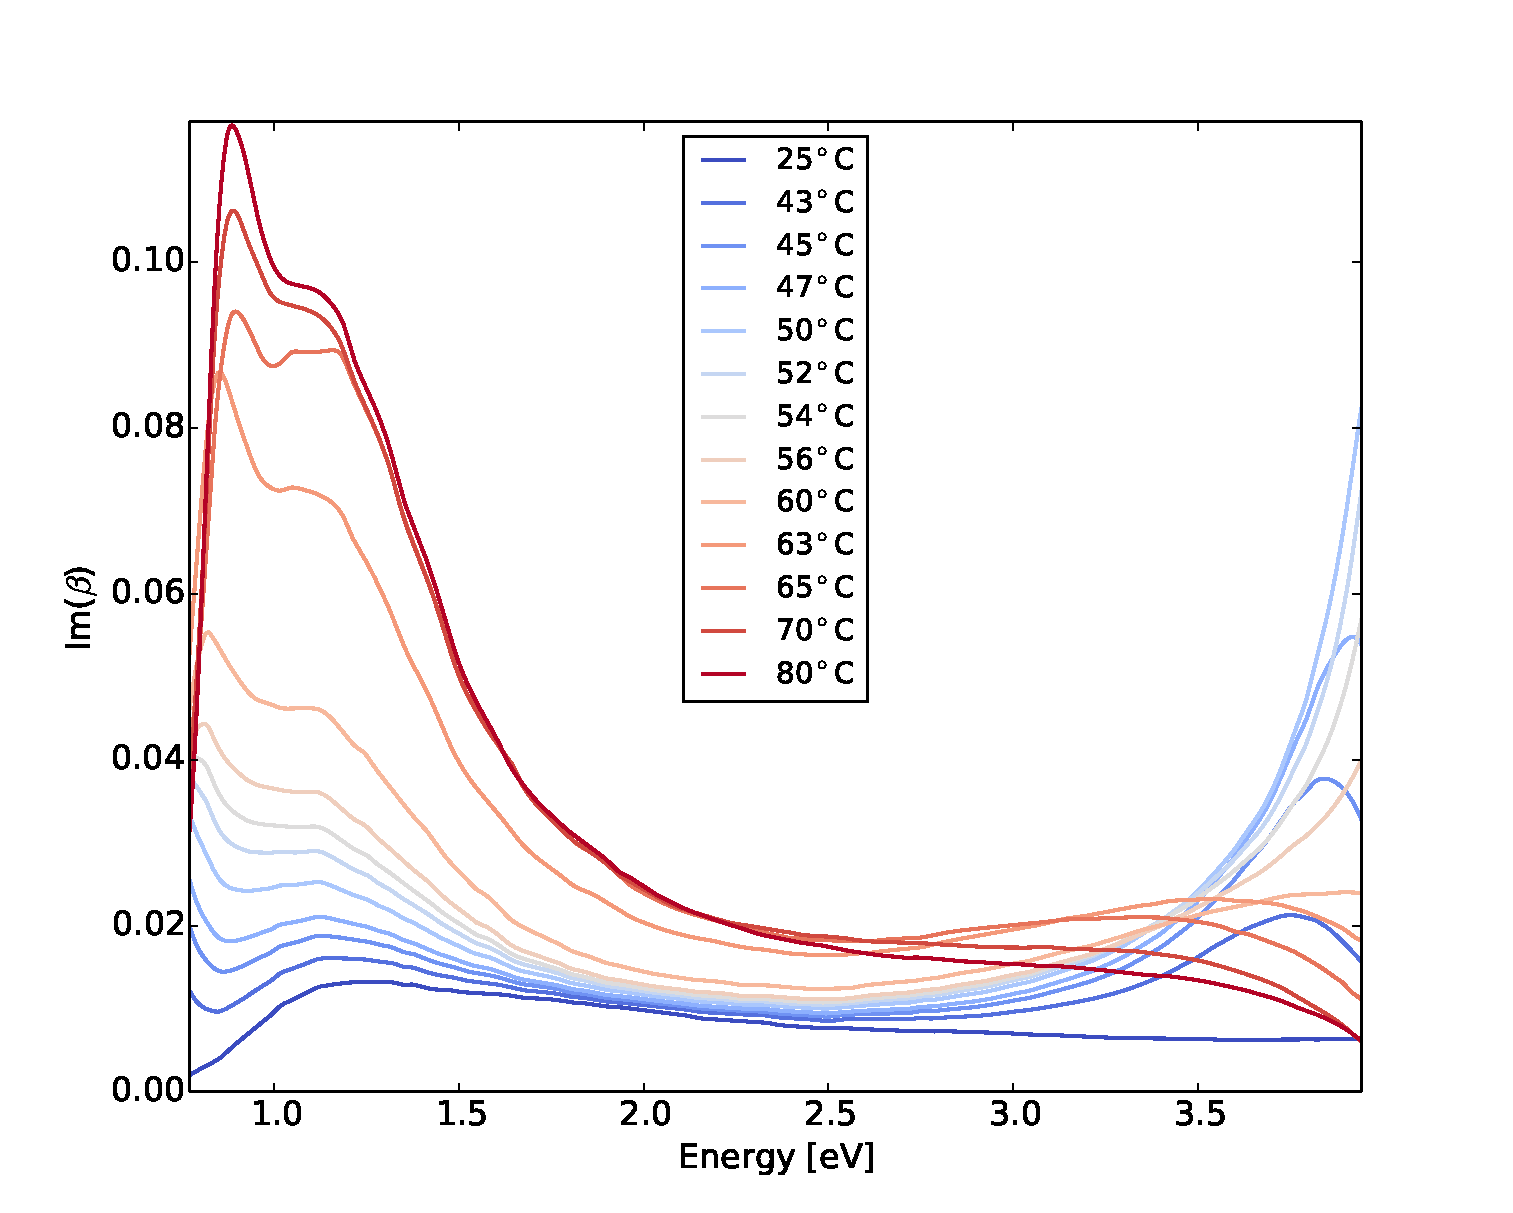
\includegraphics[width=\textwidth]{Results/Sim1/im_beta.pdf}
        \caption{}
        \label{fig:2}
    \end{subfigure}
    \caption{Relative reflectance $\Delta R/R$}
    \label{fig:}
\end{figure}
%


\section{Simulation 2; $R = 10$nm, s-polarized incident light}
\section{Simulation 3; $R = 15$nm, p-polarized incident light}
\section{Simulation 4; $R = 15$nm, s-polarized incident light}
\begin{figure}
    \centering
    \begin{subfigure}[b]{0.49\textwidth}
        \centering
        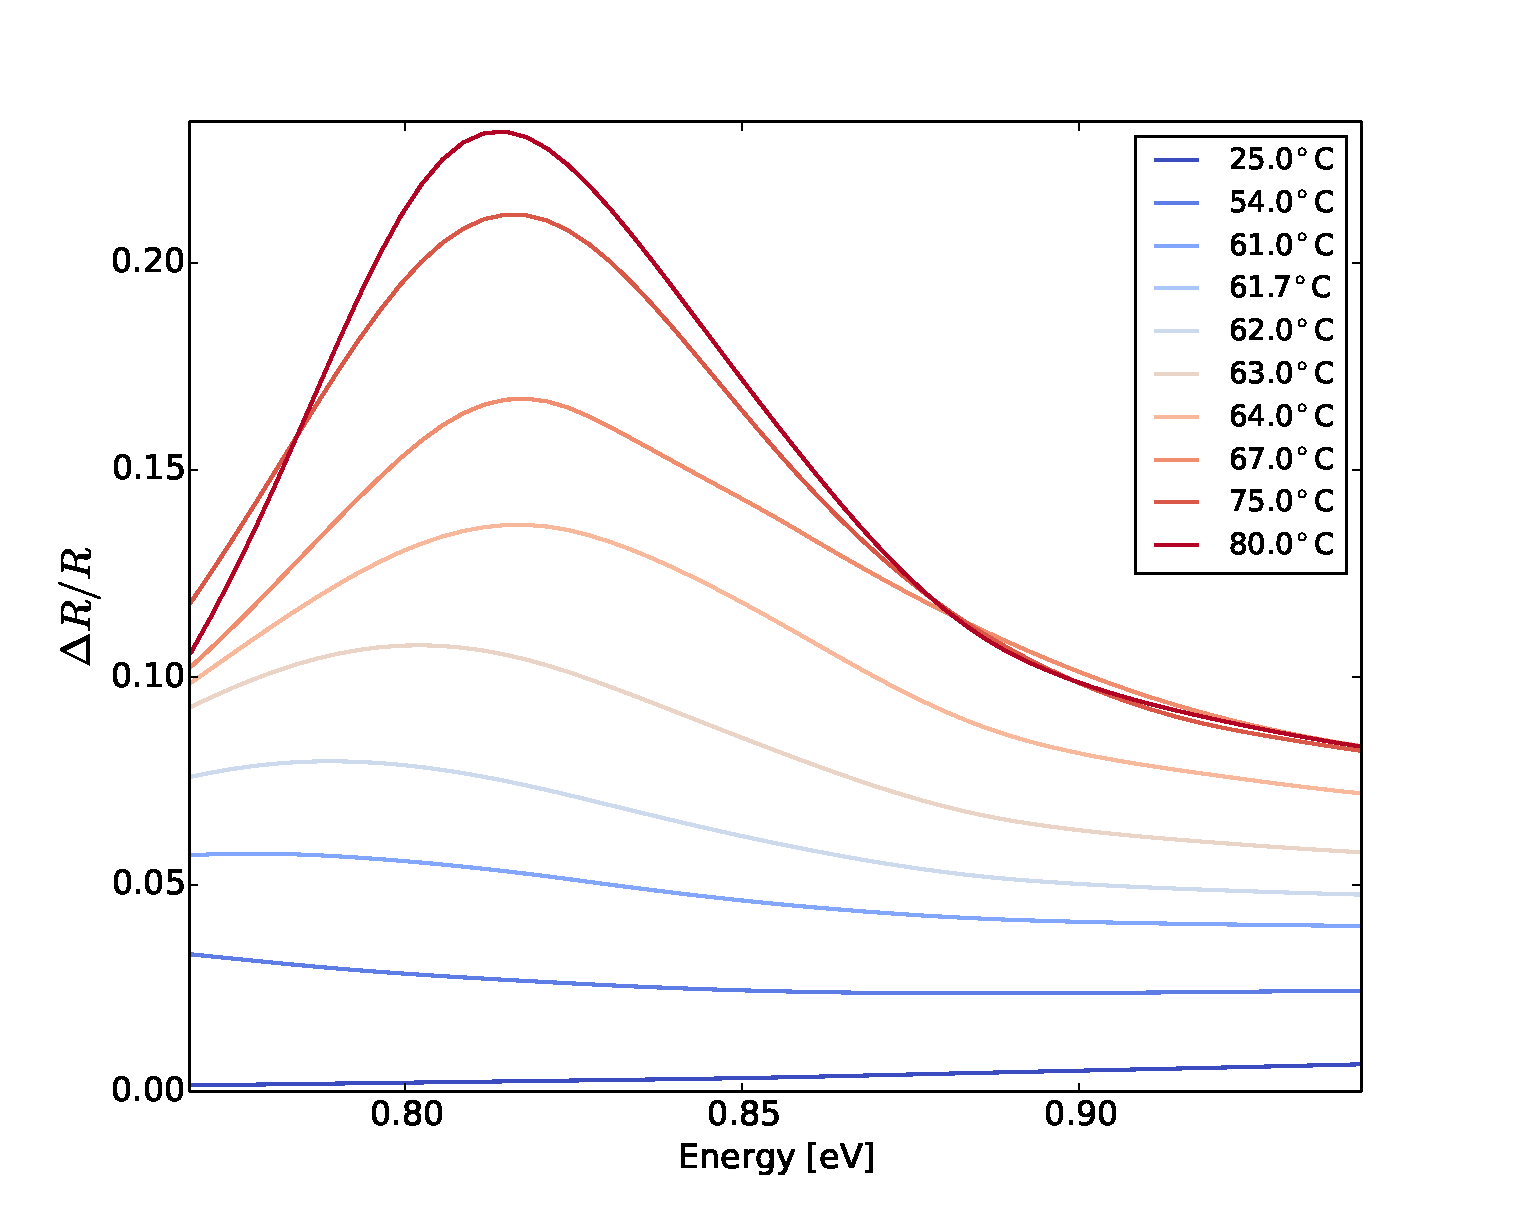
\includegraphics[width=\textwidth]{Results/Sim1/dR_lowE.pdf}
        \caption{$R=10$nm, p-polarization}
        \label{fig:y equals x}
    \end{subfigure}
    %\hfill
    \begin{subfigure}[b]{0.49\textwidth}
        \centering
        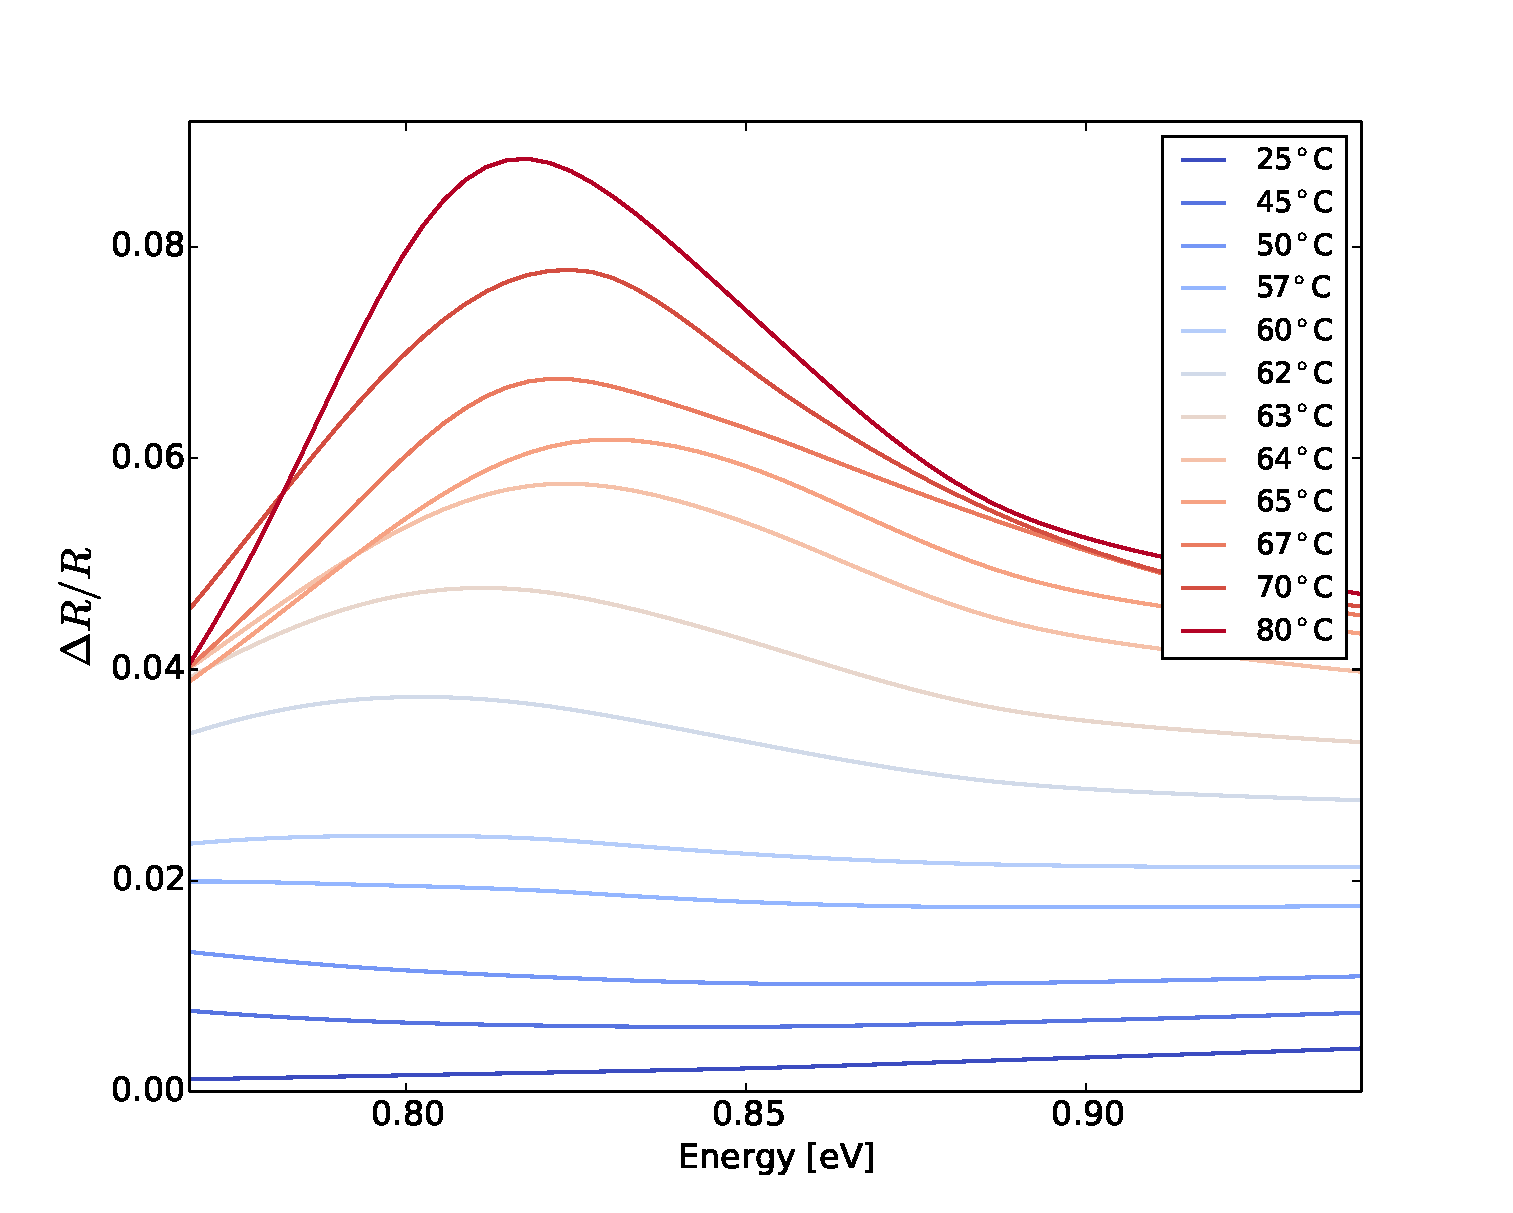
\includegraphics[width=\textwidth]{Results/Sim2/dR_lowE.pdf}
        \caption{$R=10$nm, s-polarization}
        \label{fig:five over x}
    \end{subfigure}
    %\hfill
    \begin{subfigure}[b]{0.49\textwidth}
        \centering
        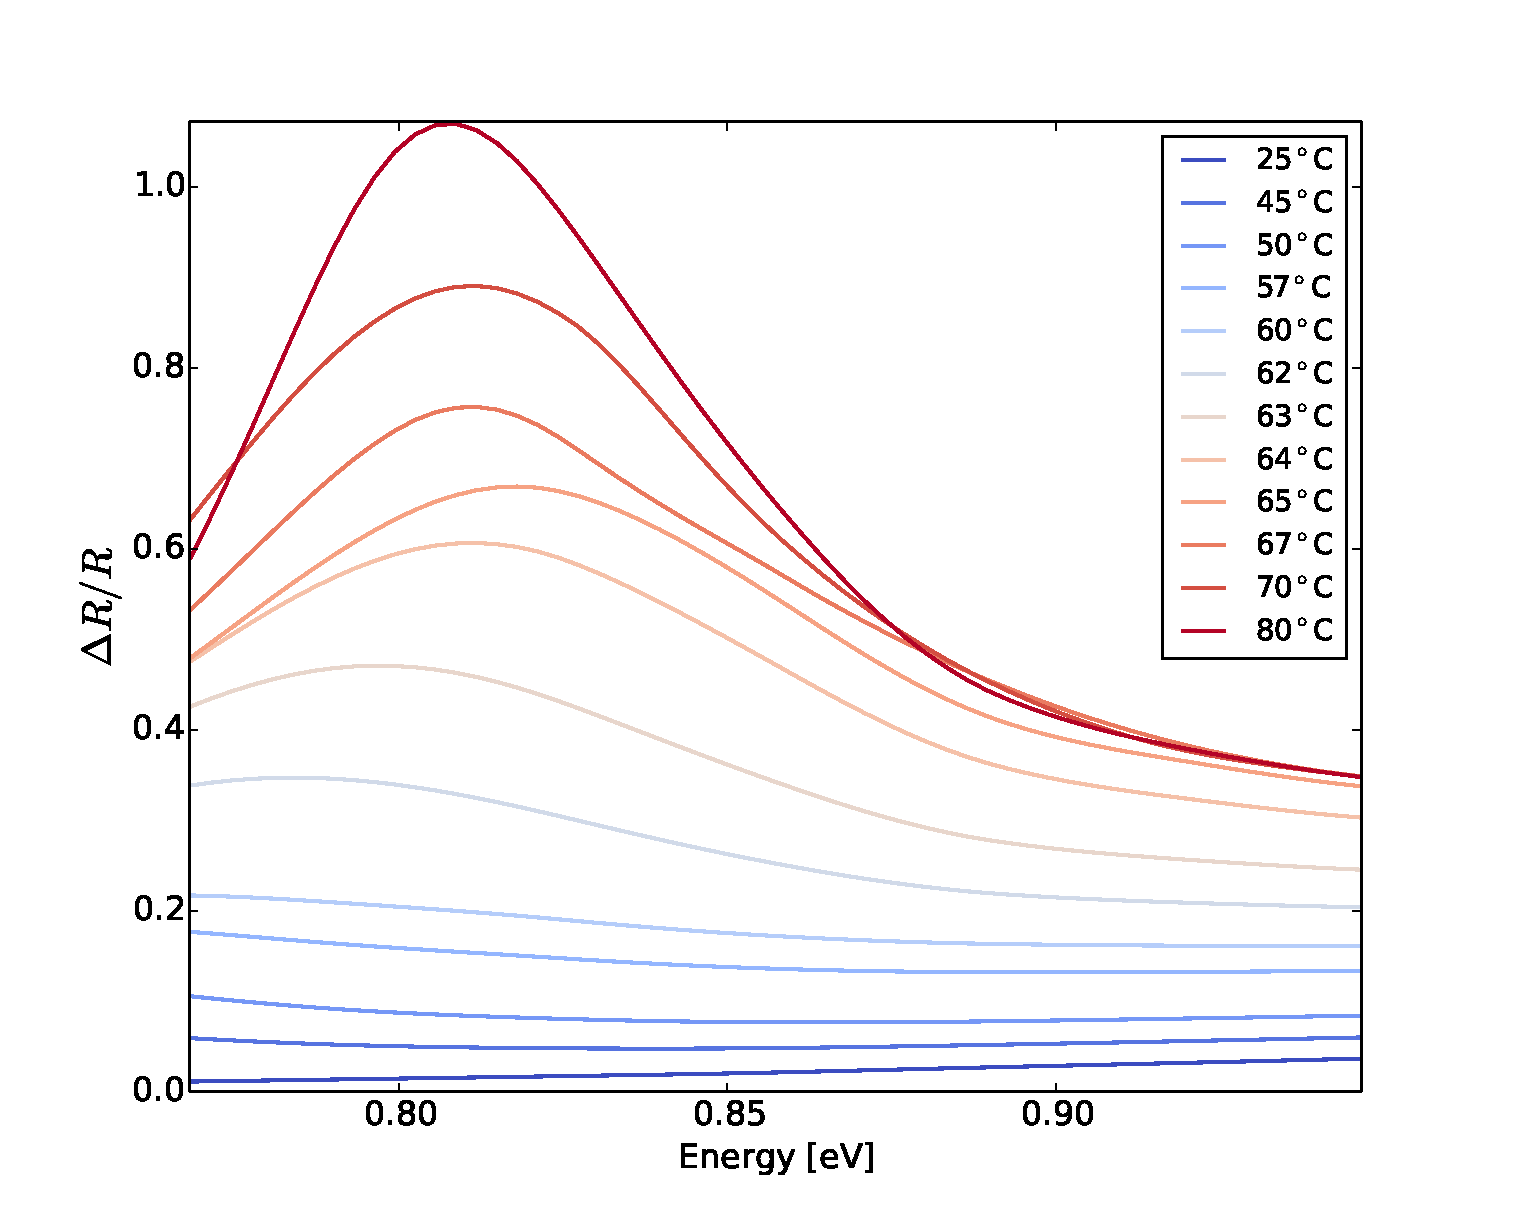
\includegraphics[width=\textwidth]{Results/Sim3/dR_lowE.pdf}
        \caption{$R=15$nm, p-polarization}
        \label{fig:three sin x}
    \end{subfigure}
    %\hfill
    \begin{subfigure}[b]{0.49\textwidth}
        \centering
        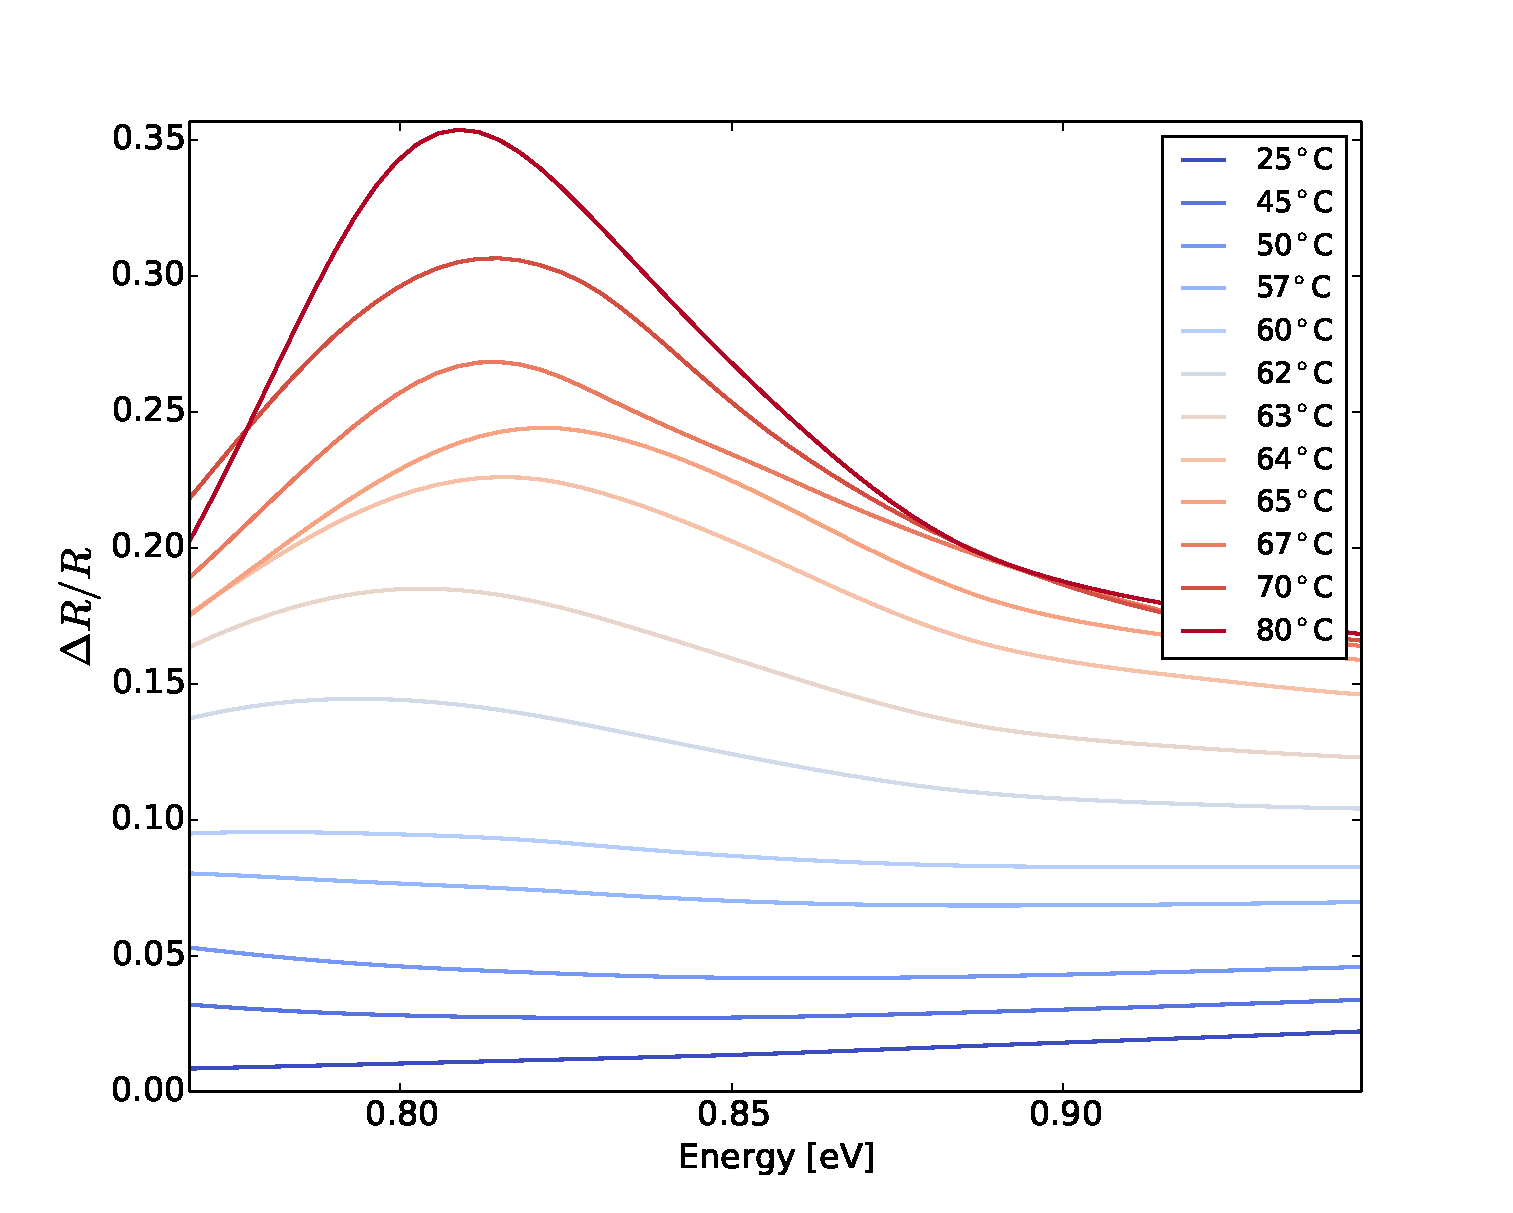
\includegraphics[width=\textwidth]{Results/Sim4/dR_lowE.pdf}
        \caption{$R=15$nm, s-polarization}
        \label{fig:five over x}
    \end{subfigure}
    \caption{Relative reflectance $\Delta R/R$}
    \label{fig:three graphs}
\end{figure}



\section{Discussion}

\section{Conclusion}


\section{Introduction to GranFilm}
This section is included as a brief summary of the practical situations one encounter
when using GranFilm. Even though the software provides the information required and would be
self-explanatory for some, this would be for the less experienced reader to avoid any unecessary 
confusion.

\subsection{Software overview}
\textsc{GranFilm} is a program written in \textsc{Fortran 90} and serves as a tool for simulating 
and interpreting optical spectra from surfaces or thin films. The program takes in parameters specifying
the incoming angle, polarization and energy range of the incoming plane wave, in addition to the
radius and truncation ratio $t_r$ of the sphere, the materials for region 1,2,3 and 4,
the arrangement of the islands and finally the multipole order $M$.  



\newpage
\section{Additional Theory}

\subsection{Complex permittivity and refractive index (From wikipedia) don't use, LACKING REFERENCES!}
Complex electric permittivity:
\begin{align}
   \hat{\varepsilon}_r(\omega) = \frac{\hat{\varepsilon} (\omega)}{\varepsilon_0}
\end{align}
where 
\begin{align}
   \hat{\varepsilon}_r(\omega) &= \varepsilon_r (\omega) + i\tilde{\varepsilon}_r (\omega) \\
                               &= \varepsilon_r (\omega) + i\frac{\sigma}{\omega\varepsilon_0} 
\end{align}
The complex refractive index $\hat{n}$ is given by 
\begin{align}
   \hat{n} = \sqrt{\hat{\varepsilon}_r},
\end{align}
when the magnetic properties are neglected ($\mu_r = 1$). 
From this, an expression for the complex refractive index $\hat{n} = n - \boldsymbol{i}\kappa$ can be found:
\begin{align}
   \hat{\varepsilon}_r &= \hat{n}^2 \\
   \varepsilon_r + \boldsymbol{i}\tilde{\varepsilon}_r &= (n + \boldsymbol{i} \kappa)^2 \\
   \varepsilon_r + \boldsymbol{i}\tilde{\varepsilon}_r &= n^2 - \kappa^2 + \boldsymbol{i}2n\kappa
\end{align}
giving
\begin{align}
   \varepsilon_r &= n^2 - \kappa^2     &\tilde{\varepsilon}_r  &= 2n\kappa.
\end{align}
Taking the absolute value or modulus of the relative permettivity
\begin{align}
   |\hat{\varepsilon}_r| &= \sqrt{ \varepsilon_r^2 + \tilde{\varepsilon}_r^2} \\
   |\hat{\varepsilon}_r| &= \sqrt{ (n^2 - \kappa^2)^2 + (2n\kappa)^2} \\
   |\hat{\varepsilon}_r|^2 &= (n^4 - 2n^2\kappa^2 + \kappa^4) + 4n^2\kappa^2 \\
   |\hat{\varepsilon}_r|^2 &= n^4 + 2n^2\kappa^2 + \kappa^4 \\
   |\hat{\varepsilon}_r|^2 &= (n^2 + \kappa^2)^2 \\
   |\hat{\varepsilon}_r| &= n^2 + \kappa^2 
\end{align}
and adding or substracting the real part of the permittivity, gives
\begin{align}
   |\hat{\varepsilon}_r| + \varepsilon_r &= (n^2 + \kappa^2) + (n^2 - \kappa^2) = 2n^2\\
   |\hat{\varepsilon}_r| - \varepsilon_r &= (n^2 + \kappa^2) - (n^2 - \kappa^2) = 2\kappa^2.
\end{align}
Refomulating the expression gives the real and imaginary parts of $\hat{n}$
\begin{align}
   n      &= \sqrt{ \frac{|\hat{\varepsilon}_r| + \varepsilon_r}{2}} 
           = \sqrt{ \frac{|\hat{\varepsilon}| + \varepsilon}{2\varepsilon_0}}\\
   \kappa &= \sqrt{ \frac{|\hat{\varepsilon}_r| - \varepsilon_r}{2}} 
           = \sqrt{ \frac{|\hat{\varepsilon}| - \varepsilon}{2\varepsilon_0}}
\end{align}


\subsection{Polarizability. Don't use, LACKING REFERENCES}
When a neutral atom is placed in an electric field $\boldsymbol{E}$, the field tries to rip the
atom apart by pushing the nucleus in the direction of the field and the electrons in the opposite direction.
Because of the attraction between the positive and negative charge within the atom, an equilibrium displacement
of the electrons compared to the nucleus is achieved, leaving the atom polarized and giving it a
dipole moment. The dipole moment can be approximated by
\begin{align}
   \boldsymbol{p} = \alpha \boldsymbol{E},
\end{align}
where $\alpha$ is the atomic polarizability and may depend on the detailed structure of the atom.
For more complicated situations, like an asymmetrical molecule, the gained dipole moment of the 
molecule does not necessarily have to be in the same direction as the applied electric field.
In such a case, the scalar polarizability in the expression above is replaced by a polarizability tensor
\begin{align}
   \boldsymbol{\alpha} = 
\begin{bmatrix}
   \alpha_{xx}   &   \alpha_{xy}  &  \alpha_{xz}  \\
   \alpha_{yx}   &   \alpha_{yy}  &  \alpha_{yz}  \\
   \alpha_{zx}   &   \alpha_{zy}  &  \alpha_{zz} 
\end{bmatrix}
.
\end{align}
In this way, an applied eletric field induces many dipole moments in a material. In addition,
any polar molecules will be subject to a torque, aligning it to the direction of the field.
These two mechanisms leads to the polarization $\boldsymbol{P}$ of the material
\begin{align}
   \boldsymbol{P} = \text{dipole moment per unit volume} = \varepsilon_0 \chi_e \boldsymbol{E}.
\end{align}
In the above expression, there has been assumed a linear dielectric media, where $\chi_e$ is the electric 
susceptibility and depends on the microscopic structure of the material, in addition to the external 
temperature (\cite{Griffiths},p.160-166, 179)

\subsection{The electric potential, Laplace's equation and the Uniqueness Theorem}
The usual task of electrostatics is to ompute the electric field $\boldsymbol{E}$ given a 
stationary charge distribution $\rho{\boldsymbol{r}}$
\begin{align}
   \boldsymbol{E}(\boldsymbol{r}) 
   &= \frac{1}{4 \pi \varepsilon_0} \int \frac{\boldsymbol{\hat{d}}(\boldsymbol{r'})}
                                              {d(\boldsymbol{r'})^2} 
                                                            \rho(\boldsymbol{r'}) d\!\boldsymbol{r'} 
                                                            \\
   &= \frac{1}{4 \pi \varepsilon_0} \int \frac{\boldsymbol{r} - \boldsymbol{r'}}
                                              {\big|\boldsymbol{r} - \boldsymbol{r'}\big|^3} 
                                                           \rho(\boldsymbol{r'}) d\!\boldsymbol{r'}.
\end{align}
However, it is usually simpler to calculate the potential
\begin{align}
   \label{electricPotential}
   V(\boldsymbol{r}) 
   &= \frac{1}{4 \pi \varepsilon_0} \int \frac{1}{\big|\boldsymbol{r} - \boldsymbol{r'}\big|} 
                                                           \rho(\boldsymbol{r'}) d\!\boldsymbol{r'}
\end{align}
first and then calculate the electric field from
\begin{align}
   \boldsymbol{E} = - \nabla V.
\end{align}
This might in some situations, where do do not necessarily know $\rho$ but only the total amount of 
charge, also be to tough to handle analytically. In situations like these it is better to use
Poisson's equation
\begin{align}
   \label{poisson}
   \nabla^2 V= - \frac{1}{\varepsilon_o} \rho,
\end{align}
which together with appropriate boundary conditions, is equivalent to Eq.\eqref{electricPotential}.
Very often, we are interested in finding the potential containing no charge (because the charge is 
located on the outside of our region of interest. In such cases Eq. \eqref{poisson} reduces to
Laplace's equation (\cite{Griffiths}, p.110-111)
\begin{align}
   \label{laplace}
   \nabla^2 V = 0.
\end{align}
According to the \textit{Uniqueness Theorems}, the solution to Laplace's equation is uniquely 
determined in some volume if the potential is specified on the boundary of the volume. This
easily extends to Poisson's equation by further requiring, in addition to the 
potential on the boundary, that the charge distribution throughout the region is known.
\\
\\
When considering conductors, charge are allowed to move freely and  might start to rearrange themselves,
leading to the \textit{Second uniqueness theorem}, which states that the potential in a given volume,
surrounded by conductors is uniquely determined if the total charge on each conductor is given.
\\
\\
The uniqueness theorem grants an enlarged mathematical freedom in the approach of finding the potential
of a region of space. This is because the boundary uniquely determines the potential in the region enclosed
region and any approach giving the correct boundary conditions would give you the correct potential 
function through Laplace's equation Eq. \eqref{laplace}. This allows the use of tricks, like for example
the classical \textit{method of images} (\cite{Griffiths}, p.116-121).
%SOME EXTRA STUFF:
%\textbf{D'Alembert Operator $\square$}
%\begin{align*}
  %\square  &= \partial ^{\mu} \partial _{\mu}
   %\\
           %&= \frac{1}{c^2} \frac{\partial ^2}{\partial t^2} 
               %- \frac{\partial ^2}{\partial x^2} 
               %- \frac{\partial ^2}{\partial y^2} 
               %- \frac{\partial ^2}{\partial z^2} 
   %\\
           %&= \frac{1}{c^2} \frac{\partial ^2}{\partial t^2} - \nabla ^2
%\end{align*}

%\textbf{Lorentz Gauge:} \\
%For Lorentz invariance, convenient to choose the Lorenz gauge:
%\begin{align*}
   %\square \vec{A} = \Bigg[ \frac{1}{c^2} \frac{\partial ^2}{\partial t^2} - \nabla ^2 \Bigg] \vec{A} = \mu_0 \vec{J}
%\end{align*}
%\begin{align*}
   %\square \phi = \Bigg[ \frac{1}{c^2} \frac{\partial ^2}{\partial t^2} - \nabla ^2 \Bigg] \phi = \frac{\rho}{\epsilon _0}
%\end{align*}


\newpage
\clearpage
\begin{thebibliography}{9}

%		\bibitem{poisson}
%		Einar M. Rønquist,
%		\emph{The Poisson problem in $\mathbb{R}^2$: Diagonalization methods},
%		Department of Mathematical Sciences,
%		NTNU,N-7491 Trondheim, Norway,
%		Revised by Arne Morten Kvarving, 2014.

      \bibitem{opticalProperties}
      D. Bedeaux, J. Vlieger, 
      \emph{Optical Properties of Surfaces}, 
      Imperial College Press, 
      London, 2001

      %\bibitem{griffiths}
      %D. J. Griffiths.
      %\emph{Introduction To Electrodynamics}.
      %???Prentice Hall, Third Edition, 2004. ???

\end{thebibliography}



%
\end{document}

